%%
%% This is file `uantwerpenbamathesis-example.tex',
%% generated with the docstrip utility.
%%
%% The original source files were:
%%
%% uantwerpendocs.dtx  (with options: `bmt-example')
%% 
%% This is a generated file.
%% 
%% Copyright (C) 2013-2022  by Walter Daems <walter.daems@uantwerpen.be>
%% 
%% This work may be distributed and/or modified under the conditions of
%% the LaTeX Project Public License, either version 1.3 of this license
%% or (at your option) any later version.  The latest version of this
%% license is in:
%% 
%%    http://www.latex-project.org/lppl.txt
%% 
%% and version 1.3 or later is part of all distributions of LaTeX version
%% 2005/12/01 or later.
%% 
%% This work has the LPPL maintenance status `maintained'.
%% 
%% The Current Maintainer of this work is Walter Daems.
%%
% !TEX root = uantwerpenbamathesis-example.tex
\documentclass[we,twoside,openright,a4paper,11pt]{uantwerpenbamathesis}
\usepackage{subcaption}
\usepackage{booktabs}
\usepackage{tcolorbox}
\usepackage{scrhack}

\usepackage[english]{babel} % or english if your text is in English
\usepackage{amsmath}

\usepackage[backref,hyperindex=true,pagebackref=true]{hyperref}
                          % New: you must load the hyperref package
                          % yourself! This allows you to put it in the
                          % correct order with the other packages you load!

\usepackage{mathptmx}
\DeclareMathAlphabet{\mathcal}{OMS}{cmsy}{m}{n}
\iftutex
\usepackage{fontspec}
\setmainfont{Calibri} % comment this line out if you want computer
                      % modern as main font, or feel free to select
                      % any other font
\setsansfont{Calibri}
\usepackage{sansmathaccent}
\fi

\usepackage{multicol}
\usepackage{float}

\bamadegree{en-pr}

\title{Exam Programming: PINN} % either don't split titles, or do so with hypen
                     % and a newline
\subtitle{Using Physics Informed Neural Networks to solve nonlinear Partial Differential Equations}
\author{Des De Borger}

\academicyear{2025 - 2026}

\begin{document}

\maketitle

\frontmatter

\tableofcontents

\mainmatter

\chapter{Introduction}

Physics-Informed Neural Networks (PINNs) are a class of machine learning models which augment standard neural network training with prior knowledge of the physical laws governing a system. Rather than learning purely from data, a PINN is simultaneously trained to minimise the residual of a governing differential equation at a set of collocation points, enforcing consistency with the underlying physics throughout the domain. This makes PINNs particularly appealing in settings where observational data is scarce, noisy, or incomplete; these conditions are common in scientific and engineering applications.

This report investigates the application of PINNs to two problems in mathematical physics. The first is the damped harmonic oscillator, a second-order ODE that describes oscillatory motion with energy dissipation (friction). The second is the one-dimensional viscid Burger's equation, a nonlinear PDE which captures the competing effects of advection and diffusion, and which exhibits the physically interesting phenomenon of shock formation and rarefaction waves.

For each problem, the report proceeds as follows. The governing equations and their analytic or numerical solutions are introduced to establish a ground truth. A PINN implementation is then developed and analysed in detail, covering the structure of the loss function, network architecture, training procedure, and hyperparameter sensitivity. Improvements over a baseline example are proposed and justified, including randomised training data, early stopping, and systematic hyperparameter optimisation using the Optuna library. Finally, the inverse problem is tackled for both systems: extracting unknown physical parameters (the damping ratio $\zeta$ and natural frequency $\omega_0$ for the oscillator, and the kinematic viscosity $\nu$ for Burger's equation) from noisy observational data.

The code for all experiments is structured in a modular, reusable fashion across the \verb|Damped_Oscillator| and \verb|Burgers_Equation| directories, and is described alongside the corresponding results throughout this report.

\chapter{Damped Harmonic Oscillator}
In this chapter, we will apply PINNs to solve the damped harmonic oscillator, a secondary order ODE which describes oscillatory motion with friction. The code for this chapter can be found in the \verb|Damped_Oscillator| directory.
\section{Analytic solution}
The central equation we are trying to solve is given by:
\begin{equation}\label{eq:damped_harmonic_oscillator}
    my''(t)+cy'(t)+ky(t)=0
\end{equation}
This is a second order linear ordinary differential equation. The formal solution of this equation can be found by substituting $y(t)=e^{rt}$ and solving the characteristic equation:
\begin{equation}\label{eq:damped_harmonic_oscillator_characteristic_equation}
     mr^2+cr+k=0
\end{equation}
The roots of this equation are given by:
\begin{equation}\label{eq:damped_harmonic_oscillator_roots}
    r_{1,2}=\frac{-c\pm\sqrt{c^2-4mk}}{2m}
\end{equation}
It can be useful to introduce the parameters $\omega_0=\sqrt{k/m}$ and $\zeta=c/(2\sqrt{mk})$, in which case the roots of the equation become:
\begin{equation}\label{eq:damped_harmonic_oscillator_roots_normalized}
    r_{1,2}=-\zeta\omega_0\pm\omega_0\sqrt{\zeta^2-1}
\end{equation}
We can distinguish three cases based on the value of the discriminant $D=c^2-4mk$ and $\zeta$. Figures \ref{fig:analytic_solution_overdamped} to \ref{fig:analytic_solution_underdamped} illustrate these cases.\\

\paragraph{Overdamped} If $D>0$ ($\zeta>1$), the roots are real and the solution is given by:
\begin{equation}\label{eq:damped_harmonic_oscillator_overdamped_solution}
    y(t)=Ae^{r_1t}+Be^{r_2t}
\end{equation}
Where $r_1,\ r_2<0$ are real and $A$ and $B$ are constants determined by the initial conditions $y(0)=y_0$ and $y'(0)=dy_0$:
\begin{equation}\label{eq:damped_harmonic_oscillator_overdamped_constants}
    \begin{split}
        A&=\frac{dy_0-r_2y_0}{r_1-r_2}\\
        B&=\frac{-dy_0+r_1y_0}{r_1-r_2}
    \end{split}
\end{equation}

\paragraph{Critically damped} if $D=0$ ($\zeta=1$), the roots $r_1=r_2=r=-\zeta\omega_0$ are negative, real and equal. A second linearly independent solution is then given by $te^{rt}$, so the generalsolution is given by:
\begin{equation}\label{eq:damped_harmonic_oscillator_critically_damped_solution}
    y(t)=(A+Bt)e^{rt}
\end{equation}
The constants $A$ and $B$ are again determined by the initial conditions:
\begin{equation}\label{eq:damped_harmonic_oscillator_critically_damped_constants}
    \begin{split}
        A&=y_0\\
        B&=dy_0-ry_0
    \end{split}
\end{equation}

\paragraph{Underdamped} if $D<0$ ($\zeta<1$), the roots $r_1$ and $r_2$ are complex conjugates, whose complex parts are conventionally expressed as $\omega_d=\omega_0\sqrt{1-\zeta^2}$, so that the roots can be expressed as $r_{1,2}=-\zeta\omega_0\pm i\omega_d$. The solution is then given by:
\begin{equation}\label{eq:damped_harmonic_oscillator_underdamped_solution}
    y(t)=e^{-\zeta\omega_0t}(A\cos(\omega_dt)+B\sin(\omega_dt))
\end{equation}
The constants $A$ and $B$ are again determined by the initial conditions:
\begin{equation}\label{eq:damped_harmonic_oscillator_underdamped_constants}
    \begin{split}
        A&=y_0\\
        B&=\frac{dy_0+\zeta\omega_0y_0}{\omega_d}
    \end{split}
\end{equation}

\begin{figure}[H]
    \centering
    \includegraphics[width=0.7\textwidth]{Images_DHO/analytic_solution_overdamped.png}
    \caption{Analytic solution for the overdamped harmonic oscillator.}
    \label{fig:analytic_solution_overdamped}
\end{figure}

\begin{figure}[H]
    \centering
    \includegraphics[width=0.7\textwidth]{Images_DHO/analytic_solution_criticallydamped.png}
    \caption{Analytic solution for the critically damped harmonic oscillator.}
    \label{fig:analytic_solution_critically_damped}
\end{figure}

\begin{figure}[H]
    \centering
    \includegraphics[width=0.7\textwidth]{Images_DHO/analytic_solution_underdamped.png}
    \caption{Analytic solution for the underdamped harmonic oscillator.}
    \label{fig:analytic_solution_underdamped}
\end{figure}


\section{Understanding the PINN example}
In this section, we will study the provided code \verb|pinn_spring_damper.py| and attempt to respond to the questions about the method and the code. The provided example trains a standard ML model and a PINN to solve the underdamped case of the damped harmonic oscillator. The models in question are trained on 15 noisy observation points, which are supplemented with the initial conditions and the physics residual al 200 evenly spaced collocation points in the case for the PINN.

\subsection{Questions on the method}

\begin{tcolorbox}[title=Question 1, colback=blue!10!white, colframe=blue!40!white, sharp corners]
    Identify the total loss function in the code and write its expression down in your report. Identify the different contributions to the loss function.
\end{tcolorbox}
The total loss function has three terms and is displayed below:
\begin{equation}\label{eq:loss_total_DHO}
    \mathcal{L}_{tot}=\mathcal{L}_{data}+\lambda_{physics}\mathcal{L}_{physics}+\lambda_{i.c.}\mathcal{L}_{i.c.}
\end{equation}

The first term is the mean squared error of the predicted data compared to the 15 noisy observation points:
\begin{equation}\label{eq:loss_data_DHO}
    \mathcal{L}_{data}=\frac{1}{M}\sum_{j=1}^M \left(\hat{y}(t_j)-y_j\right)^2
\end{equation}
with $j=1, 2, \ldots 15$. This term is the total loss function of a standard, non-PI NN and gives the model direct information about the correct solution of the equation with the relevant boundary conditions, but doesn't check for any non-physical behavior.\\

The second term is the mean squared residual of the ODE (see equation \ref{eq:damped_harmonic_oscillator}) at the 200 evenly spaced collocation points:
\begin{equation}\label{eq:loss_physics_DHO}
    \mathcal{L}_{physics}=\frac{1}{N}\sum_{i=1}^N \left(m\hat{y}''(t_i)+c\hat{y}'(t_i)+k\hat{y}(t_i)\right)^2
\end{equation}
with $i=1, 2, \ldots 200$. This term gives the model information about how much the predicted solution violates the mechanics of the system, without checking if the predicted solution matches the observed data.\\

The third term is the sum of squared errors of the two inital conditions:
\begin{equation}\label{eq:loss_i.c._DHO}
    \mathcal{L}_{i.c.}=\left(\hat{y}(0)-y_0\right)^2+\left(\hat{y}'(0)-dy_0\right)^2
\end{equation}
This term enforces the initial conditions and applies only to the very first point $t=0$.\\

The constants $\lambda_{physics}$ and $\lambda_{i.c.}$ determine the relative weight of every term in the loss function. Because it is important that the initial conditions are met, $\lambda_{i.c.}$ is chosen at a much larger value than $\lambda_{physics}$. This is why in the given program, the values are set at $\lambda_{physics}=0.01$ and $\lambda_{i.c.}=10$.


\begin{tcolorbox}[title=Question 2, colback=blue!10!white, colframe=blue!40!white, sharp corners]
    Is the inclusion of the initial condition loss essential for this particular example? When would it be essential?
\end{tcolorbox}

To investigate the effect of the initial condition term, the term can be dropped out of the loss function to compare the results. Figure \ref{fig:ic_comp} shows the predicted solutions of the ODE if the $\mathcal{L}_{i.c.}$ is included and excluded. In this specific case, there does not seem to be a big difference which indicated that the initial condition loss is not essential. This is because the noisy observations point, which also contribute to the loss function, are close enough to $t=0$ to give enough information for the model to accurately predict the initial conditions.

\begin{figure}[H]
    \centering
    \includegraphics[width=0.75\textwidth]{Images_DHO/ic_effect.png}
    \caption{Predicted solutions to the ODE of the $\mathcal{L}_{i.c.}$ is included and excluded. In this specific case, the $\mathcal{L}_{i.c.}$ is not absolutely necessary, because the noisy observation points give enoug information for the model to accurately predict the initial conditions.}
    \label{fig:ic_comp}
\end{figure}

We do not always have access to observations close to the initial time $t_0$. However, if the initial conditions are known and need to be enforced, $\mathcal{L}_{i.c.}$ is a crucial term in the total loss function. 

\begin{tcolorbox}[title=Question 3, colback=blue!10!white, colframe=blue!40!white, sharp corners]
    The loss function used here is based on the mean squared errors (MSE) between predictions and data points or initial condition, and on the mean squared residual (MSR) of the PDE for the collocation points. Why are these specific functional forms used, and would there be alternative functions that could replace the MSE or MSR?
\end{tcolorbox}

The mean square error and mean square residuals are the most commonly used loss functions for regression models. Any loss function has to be symmetrical and positive for all possible values, so that errors cannot cancel each other out. Furthermore, it is desired that the loss function is differentiable so that its gradient can be computed.\\

The MSE and MSR check both of these boxes. However, since the errors are squared before averaging, these functions heavily punish and are sensitive to large outliers. This can lead to problems when very noisy data points are included in the calculation for the loss function. However, this effect is good for the residuals since it is essential that the predicted solution does not break the laws of physics. There are alternative loss functions with different (dis)advantages \cite{geeksforgeeks2024lossfunctions}:\\
\paragraph{Mean Absolute Error} The Mean Absolute Error (MAE) does not average the squares, but the absolute distances:
\begin{equation}\label{eq:loss_MAE}
    \mathcal{L}_{MAE}=\frac{1}{M}\sum_{j=1}^M \left|\hat{y}(t_j)-y_j\right|
\end{equation}
Because the errors are not squared, this loss function is less sensitive to large outliers, which can make it more robust. However, it is not differentiable at zero, which can lead to problems for some optimisation algorithms.

\paragraph{Huber Loss} The Huber Loss is a hybrid of the MAE and the MSE which is differentiable, but less sensitive to ouliers than the MSE. It is defined as follows:
\begin{equation}\label{eq:huber_loss}
    L_{\delta}(x) = \begin{cases}
        \frac{1}{2}x^2 & \text{if } |x| \leq \delta \\
        \delta\left(|x| - \frac{1}{2}\delta\right) & \text{if } |x| \geq \delta
    \end{cases}
\end{equation}
The Huber Loss behaves like the MSE for $|x|<\delta$ and like the MAE for $|x|>\delta$. The hyperparameter $\delta$ can be tuned to make the loss function more or less sensitive to outliers.

\begin{tcolorbox}[title=Question 4, colback=blue!10!white, colframe=blue!40!white, sharp corners]
    What is the type of neural network used in this example? How many input nodes, output nodes and hidden layers does it have? How many parameters are then being optimized? What type of activation function is used and why? What quantity or quantities are provided at the input, and what quantity or quantities do we extract from the output of the network? Are the dimensions of this Neural Network architecture adequate, too small or too large for this example? How would you determine this?
\end{tcolorbox}

We are trying to solve an ODE, which means to solve for a function $y(t)$. This function takes one input and returns one output, which means the network will also need to have one input and one output, representing the time and the function value respectively.\\

A dense network is used in this specific case. The parameters for the hidden layers can be given as inputs, in the example script there are 4 hidden layers of 32 nodes. For every connection between nodes has a weight, and every node (except the input) has a bias. From this we can calculate the total parameter count:
\begin{equation}
\begin{split}
n ={}& \text{First layer weights} + \text{First layer bias} \\
     &+ \text{Hidden layer weights} + \text{Hidden layer bias} \\
     &+ \text{Last layer weights} + \text{Last layer bias} \\
     ={}&(1\cdot32 + 32) + 3(32\cdot32+32) + (1\cdot32 + 1)=3265\ \text{parameters} 
\end{split}
\end{equation}

The dimensions of the network (the depth and layer size) are hyperparameters which should be tuned according to the specific problem needs to be solved by the model. Defining the optimal value for hyperparameters such as the dimensions is a relatively subjective and empirical process, since there are no general formulas that give the optimal hyperparameter set for every problem.\\

The activation function used is a $\tanh$ function. This choice is important; we will be calculating the first and second derivatives of the output $y$ with respect to the input $t$, which means the activation function needs to be differentiable at least twice. for this reason, ex. ReLu is not suitable for this network.\\

Judging from the predicted solution, the model is large enough to make an accurate prediction for the solution to the equation. To optimise the network dimensions further, one can choose to implement an optimising algorithm which tunes the hyperparameters based on a validation set. This way, the acuraccy and training time can be optimised in a reproducible way \cite{geeksforgeeks2026hyperparameter}. Examples possible methods include:
\begin{itemize}
    \item Random search: for every hyperparameter, a range of evenly spaced values is defined. A model is trained for every single possible combination and their performances are compared.
    \item Random search: hyperparameter sets are chosen at random with user-defined ranges, and the best performing model is chosen from the resulting set of models.
    \item Bayesian optimization: a probabilistic sequential algorithm that optimises an unknown, computationally heavy function (such as the model performance).
\end{itemize}


\begin{tcolorbox}[title=Question 5, colback=blue!10!white, colframe=blue!40!white, sharp corners]
    How many input samples are provided to the neural network model during each of its training cycles or epochs? What kind of samples are provided? Does the network receive again for each epoch the same exact samples? Would there be a better way to provide samples to this network for training over the various epochs?
\end{tcolorbox}

The model receives the same 15 noisy observation points every singe epoch. These points are used to calculate $\mathcal{L}_{data}$. Furthermore, the model receives the initial conditions to calculate $\mathcal{L}_{i.c.}$. The $\mathcal{L}_{physics}$ is calculated only using the residual of equation \ref{eq:damped_harmonic_oscillator}, for which no inputs are needed.\\

This is a suboptimal approach, since the model could simply memorize the 15 given points. A better approach would be to randomize the 15 points every epoch to avoid overtraining on a specific dataset. 

% Furthermore, it would also be good practise to stop the inputting of datapoints after a defined number of epochs, so that the model is solely trained based on the equation residuals. This is even an even safer approach to avoid overtraining and is known as \textit{curriculum training}. \cite{guo2025ctlpinn}

\begin{tcolorbox}[title=Question 6, colback=blue!10!white, colframe=blue!40!white, sharp corners]
    The example uses the Adam algorithm as the so-called optimizer. What is the purpose of this optimizer? What is specific about the Adam algorithm, and what are its main hyper-parameters? Are there viable alternatives for the Adam optimizer?
\end{tcolorbox}

An optimizer is a tool to accelerate the gradient descent by taking previously calculated gradients into account \cite{geeksforgeeks2025adam}. This way, the optimizer can avoid oscillations and avoid local minima. Adam is actually a combination of two alternative optimisers:
\begin{enumerate}
    \item Momentum-based optimising \cite{geeksforgeeks2025momentum}: this technische incorporates the gradients of previous epochs by calculating an exponentially weighted moving average. If the gradient at epoch $t$ is given by $w_t$, the momentum-based gradient $m_t$ is calculated iteratively as follows:
    \begin{equation}
        m_t=\beta m_{t-1} + (1-\beta)\nabla_{w_t}\mathcal{L}_{tot}
    \end{equation}
    where $\beta$ is the momentum factor, typically chosen as 0.9. This parameter determines how much the previous gradients need to be taken into account. The weights are then updated:
    \begin{equation}
        w_t=w_{t-1}-\alpha m_t
    \end{equation}
    \item Root Mean Square Propagation \cite{geeksforgeeks2025rmsprop}: this technique uses an exponentially weighted moving average of squared gradients to optimise the learning rate $\alpha$. The learning rate is divided by a factor $\sqrt{v_t}$, the root (weighted)mean square of the gradients. This is also calculated iteratively:
    \begin{equation}
        v_t=\gamma v_{t-1}+(1-\gamma)\left(\nabla_{w_t}\mathcal{L}_{tot}\right)^2
    \end{equation}
     The weights are then updated:
    \begin{equation}
        w_t=w_{t-1}-\frac{\alpha}{\sqrt{v_t}+\epsilon} \nabla_{w_t}\mathcal{L}_{tot}
    \end{equation}
    A small value is added in the denominator to avoid division by zero.
\end{enumerate}

Both $m$ and $v$ are biased towards zero since they are initialized at zero. They need to be corrected:
\begin{equation}
    \begin{split}
        \hat m_t&=\frac{m_t}{1-\beta^t}\\
        \hat v_t&=\frac{v_t}{1-\gamma^t}\\
    \end{split}
\end{equation}

The Adam optimiser combines these two techniques and updates the weights as follows:
\begin{equation}\label{eq:adam_update}
    w_t=w_{t-1}-\frac{\alpha}{\sqrt{\hat v_t}+\epsilon} \hat m_t
\end{equation}
The Adam optimiser is widely used since it generally has an efficient performance with relative little hyperparameters; only $\alpha$, $\beta$, and $\gamma$ need to be defined. Both the learning rate and the gradient itself are made adaptive which helps to find the global minimum of the loss function more effectively. Anternative optimisers inlcude the momentum-based and RMSprop techniques as discussed above, or Adamax (a variant of Adam based on the infinity norm) and Adagrad (which accumulated the gradients instead of using the weighted average).

\begin{tcolorbox}[title=Question 7, colback=blue!10!white, colframe=blue!40!white, sharp corners]
    The example also uses an additional optimizer: a learning rate scheduler. What does this scheduler do? Is is a necessary ingredient for training a neural network? What are its main hyper-parameters? Are there alternatives that can be usefully applied in this example?
\end{tcolorbox}
The learning rate scheduler StepLR reduces the the learning rate with a factor $\gamma$ after every $n$ epochs, which are tunable hyperparameters. This adds a global decay, which can optimize the convergence in the different stages of optimisation. When the number of epochs is still small and the parameter set is still far from the optimum, the learning rate is big, but as the number of epochs gets bigger and the network converges towards the best set of parameters, the learning rate has to decrease as well in order to avoid oscillations around the minimum. This approach lead to a further acceleration of the gradient descent.\\

There exist many different alternative learning rate schedulers, such as:
\begin{enumerate}
    \item ExponentialLR: similar to StepRL but apllies a small decay factor $\gamma$ after every epoch, leading to an exponentially decreasing learning rate.
    \item CosineAnnealingLR: the learning rate follows a cosine curve which converges to a minimum value.
    \item ReduceLROnPlateau: adaptive scheduler which applies a decay factor $\gamma$ when improvement stagnates.
    \item CyclicalLR: non-traditional learning rate scheduler which periodically increases and decreases the learning rate in order to avoid local minima.
\end{enumerate}
In this specific case, StepLR or ExponentialLR are good choices to effectively train the model. 

\begin{tcolorbox}[title=Question 8, colback=blue!10!white, colframe=blue!40!white, sharp corners]
    How many epochs is the network trained for? How would you determine whether you have trained for too little or too many epochs?
\end{tcolorbox}
The model is trained for $8000$ epochs. In order to determine if this is too many/too little, we need to compare the test and training loss function curves as a function of the number of epochs. When these two curves start to diverge, it means the model is overfitting on the training set. The model is then learning meaningless details in the test set. In the provided script no validation dataset is implemented, which makes it impossible to detect overfitting in this way. A proper implementation would reserve a separate set of points, unseen during training, against which the loss is evaluated each epoch.

\begin{tcolorbox}[title=Question 9, colback=blue!10!white, colframe=blue!40!white, sharp corners]
    Would it make sense to have a set of validation points? How would these look like? How would you use them?
\end{tcolorbox}
This script does not have a set of validation points, which makes it difficult to gauge the accuracy of the model while taking the possibility of overtraining into account. The most representative way to determine the accuracy of the solution is to compare it directly to the analytic, exact solution. This can be done by defining a set of many evenly spaced values fot $t$ and calculating the analytic solution $y(t)$ at these points. This acts as the ground truth of the model. Then, the MSR between the predicted and ground truth datapoints can be calculated to give an idea of the accuracy of the model.\\

It could also be wise to split the validation points into two sets in order to more specifically invesitgate the models ability to extrapolate beyond the range in which observation points were supplied. The set would then be split up into a set of extrapolated and non-extrapolated points. Then, the mean squared errors of both sets can be compared to analyse how much worse the predictions for the extrapolated region are.

\subsection{Questions on the code}
\begin{tcolorbox}[title=Question 1, colback=blue!10!white, colframe=blue!40!white, sharp corners]
    Why are these two lines of code good, or bad, for:
    \begin{tcolorbox}[colback=gray!10!white, colframe=gray!40!white]
        \verb|torch.manual_seed(42)|\\
        \verb|np.random.seed(42)|
    \end{tcolorbox}
\end{tcolorbox}
These lines of code set the seed for the random number generation in the script. Using the same seed every time makes it so that the noisy observation points are exactly the same when the script is ran. This can make it easier to debug the script when a specific combination of observation points causes a bug.\\

It is however also important to occasionally test the script with different seeds. The model architecture and the script could become optimised for this specific seed if other seeds are never tested.

\begin{tcolorbox}[title=Question 2, colback=blue!10!white, colframe=blue!40!white, sharp corners]
    What is the purpose of the \verb|np.ndarray| statements in this function definition:
    \begin{tcolorbox}[colback=gray!10!white, colframe=gray!40!white]
        \verb|def analytic(t: np.ndarray) -> np.ndarray:|
    \end{tcolorbox}
\end{tcolorbox}

This is Python's type annotation syntax, as prescribed by PEP484 \cite{pep484}. It tells the user which datatypes the input and output need to be. No typechecking happens at runtime, so this statement doesn't explicitly raise a TypeError if an object of the wrong type is passed. It serves as dowumentation and can help the developer to keep track of the precise definitions of every variable.

\begin{tcolorbox}[title=Question 3, colback=blue!10!white, colframe=blue!40!white, sharp corners]
    The data points are created randomly and then sorted before being offered to the neural net, using this statement:
    \begin{tcolorbox}[colback=gray!10!white, colframe=gray!40!white]
        \verb|t_obs = np.sort(np.random.uniform(0.1, T_TRAIN, N_OBS))|
    \end{tcolorbox}
    Is this good or bad?
\end{tcolorbox}

Randomizing the datapoints is good practise. A periodic set of points could lead the model to memorize specific patterns, instead of predicting the general solution to the initial condition. However, as said before, this script always passes the same set of random points which negates the advantage of randomizing the points in the firs place.\\

The sorting of the points has no effect, since we are taking the MSE between the observation points and predicted points. The order in which the errors are summed has no effect on the loss function.

\begin{tcolorbox}[title=Question 4, colback=blue!10!white, colframe=blue!40!white, sharp corners]
    The collocation points are created uniformly on a fixed grid, using this statement:
    \begin{tcolorbox}[colback=gray!10!white, colframe=gray!40!white]
        \verb|t_col = np.linspace(0.0, T_EXTRAP, N_COL)|
    \end{tcolorbox}
    Is this good or bad?
\end{tcolorbox}

Using a uniform grid for the collocation points is not optimal, the model can fine-tune to the specific spacing of the collocation grid which is not desirable. It is better practise to generate the collocation points randomly at every epoch. By constantly regenerating a set of collocation points, any bias towards one region is also avoided.

\begin{tcolorbox}[title=Questions 5 and 6, colback=blue!10!white, colframe=blue!40!white, sharp corners]
    What is this statement doing? Is it necessary?
    \begin{tcolorbox}[colback=gray!10!white, colframe=gray!40!white]
        \verb|optimiser.zero_grad()|
    \end{tcolorbox}
    What are these statements doing in the training cycle? Is their order important?
    \begin{tcolorbox}[colback=gray!10!white, colframe=gray!40!white]
        \verb|loss_total.backward()|\\
        \verb|optimiser.step()|\\
        \verb|scheduler.step()|
    \end{tcolorbox}
\end{tcolorbox}
This sequence of commands updates the model weights by calculating the gradients through backpropagation. \verb|loss_total| is a $0$-dimensional PyTorch tensor representing the loss function. The \verb|loss_total.backward()| command will do a backward pass to see how the loss function changes with the model parameters (weights and biases), and apply the chain rule at every step in the calculation of \verb|loss_total|. This results in a gradient which is \textit{added} to the \verb|.grad| attribute of every parameter. In other words, \verb|loss_total.backward()| does not \textit{save} the gradient, but \textit{accumulates} the gradient. This means that the \verb|.grad| attributes need to be set to zero before every backwards pass, which is exaclty what \verb|optimiser.zero_grad()| accomplishes. This statement is absolutely necessary, without it the gradients would be accumulated in the \verb|.grad| attributes which causes the weights and biases to be updated incorrectly.\\

\verb|optimiser.step()| will read the \verb|.grad| attributes and update the $m_t$ and $v_t$ values for every parameter and update the parameters accordingly (see eq. \ref{eq:adam_update}). $m_t$ and $v_t$ are not zeroed by the \verb|optimiser.zero_grad()| command, because otherwise it would be impossible to implement the Adam optimiser since the gradients at previous epochs are needed.\\

\verb|scheduler.step()| changes the learning rate according to the specific scheduler used. In this case, an internal counter of the number of epochs is kept, and once this counter reaches a multiple of $3000$, the learning rate is halved.\\

The order of these commands are crucial. The gradients must be set to zero first to avoid accumulation of gradients. The gradients must then be calculated to avoid using the gradients of the previous epoch to update the parameters. Finally, the fresh gradients are used to update the parameters. \cite{pytorch2025}

\begin{tcolorbox}[title=Question 7, colback=blue!10!white, colframe=blue!40!white, sharp corners]
    Why do the collocation time input tensor and the initial condition time input tensor require the gradient option, while the input data tensors do not require a gradient?
    \begin{tcolorbox}[colback=gray!10!white, colframe=gray!40!white]
        \verb|t_obs_t = to_tensor(t_obs)|\\
        \verb|y_obs_t = to_tensor(y_obs)|\\
        \verb|t_col_t = to_tensor(t_col, requires_grad=True)|\\
        \verb|t_ic_t  = to_tensor(t_ic,  requires_grad=True)|
    \end{tcolorbox}
\end{tcolorbox}
The collocation points are used to calculate the MSR of the ODE as shown in equation \ref{eq:loss_physics_DHO}, and the initial conditions are used to calculate the deviation from the predicted initial conditions as shown in equation \ref{eq:loss_i.c._DHO}. In both expressions of the loss function, the derivatives of $y(t)$ show up, so these need to be calculated.\\

Rather than using finite differences to calculate the derivatives at the collocation points and at $t=0$, we can calculate the gradients during the forward pass through the model using \verb|torch.autograd.grad|. This is more efficient since it allows for the simultaneous prediction of $y(t)$ and the calculation of the derivatives. However, we need to tell the model which derivatives with respect to $t$ are required, which is done by the \verb|requires_grad=True| statement. For the calculation of the MSE of the noisy observation points as in equation \ref{eq:loss_data_DHO}, no derivatives are needed, so the statement is omitted and \verb|requires_grad| is set to the standard value \verb|False|. \cite{pytorch2025}

\begin{tcolorbox}[title=Question 8, colback=blue!10!white, colframe=blue!40!white, sharp corners]
When presenting arrays of time points to the input of my neural network, I need to convert them into a pytorch tensor, using this helper function:
\begin{tcolorbox}[colback=gray!10!white, colframe=gray!40!white]
\begin{verbatim}
def to_tensor(arr, requires_grad=False):
    return torch.tensor(arr, dtype=torch.float32,
                        requires_grad=requires_grad).unsqueeze(1)
\end{verbatim}
\end{tcolorbox}
What does the \verb|unsqueeze(1)| method of the torch.tensor class do, and why do I need to do this?
\end{tcolorbox}
The \verb|unsqueeze()| method takes a pytorch tensor of rank $n$ and adds a dimension of depth $1$ at a specified index, as shown on Figure \ref{fig:unsqueeze}. In this case, the helper function takes in a one-dimensional array of length $n$ and returns a $(n, 1)$ \verb|torch.tensor| class. This is necessary for two different reasons:
\begin{enumerate}
    \item The time arrays (\verb|t_obs_t| and \verb|t_col_t|) which are used as inputs for forward passes through the network need to be $(n, 1)$ shaped in order to do matrix multiplication. The first \verb|nn.Linear(1, 32)| layer of the network performs the following matrix multiplication:
    \begin{equation}
        y=xW^T+b
    \end{equation}
    where $x$ is the $n\times 1$ input of the first layer, consisting of $n$ samples with $1$ feature, which is the time value $t$. $W$ and $b$ are $(32\times 1)$ column matrices containing the weights and biases\footnote{$b$ cannot actually be added directly to $xW^T$ since the dimensions do not match. $b$ is actually added to each row of the $xW^T$ matrix.} of the layer and $y$ is the $n\times 32$ output. If we do not unsqueeze the time arrays, which correspond to $x$ in this case, \verb|nn.Linear(1, 32)| will interpret the $(n,)$ tensors as $(1, n)$ tensors, consisting of $1$ sample with $n$ features. This makes the matrix multiplication $xW^T$, which is $(1, n)\times(1, n)$ impossible. Note that the \verb|t_ic_t| tensor does not need to be unsqueezed, since it is a $(1,)$ shaped tensor which cannot be interpreted incorrectly by the \verb|nn.Linear(1, 32)| layer.
    \item The \verb|y_obs_t| unsqueezed tensor is not passed through the network, but rather is used to calculate the data loss $\mathcal{L}_{data}$ (see equation \ref{eq:loss_data_DHO}). When predicting the $y$ values for the \verb|t_obs_t| values, the model returns a $(n, 1)$ tensor (\verb|y_pred|). In the code, the residual is calculated as \verb|l_data = torch.mean((y_pred - y_obs_t) ** 2)|. If \verb|y_obs_t| is not unsqueezed ($(n,)$ tensor), the $(n, 1)-(n,)$ operation will return a $(n, n)$ tensor, containing \textit{all} differences $\hat y_i-y_j$, instead of only the relevant errors $\hat y_i-y_i$. When averaging over these elements using \verb|torch.mean|, it is averaging over differences and returns a loss which is not correct.
\end{enumerate}

\begin{figure}[H]
    \centering
    \includegraphics[width=0.75\textwidth]{Images_DHO/unsqueeze.png}
    \caption{Unsqueezing of a $2\times2$ tensor into $1\times2\times2$,  $2\times1\times2$, and $2\times2\times1$ tensors by using the  \texttt{unsqueeze()} method of the \texttt{torch.tensor} class.  \cite{so_unsqueeze2019}}
    \label{fig:unsqueeze}
\end{figure}


\begin{tcolorbox}[title=Question 9, colback=blue!10!white, colframe=blue!40!white, sharp corners]
    When computing the first and second derivatives of $y(t)$ we use the \verb|torch.autograd| method. Explain why the \verb|grad_outputs| are set to ones and why we need to take the zero-th element \verb|[0]| of this output in the statements below:
    \begin{tcolorbox}[colback=gray!10!white, colframe=gray!40!white]
        \verb|dy = torch.autograd.grad(|\\
        \verb|    y_hat, t,|\\
        \verb|    grad_outputs=torch.ones_like(y_hat),|\\
        \verb|    create_graph=True)[0]|
    \end{tcolorbox}
\end{tcolorbox}
The \verb|torch.autograd.grad| differentiates an output vector $y=(y_1, \ldots, y_n)$ with respect to an input vector $t=(t_1, \ldots, t_n)$ and returns a vector-Jacobian product:
\begin{equation}
    v^TJ =  v^T
    \begin{pmatrix}
        \frac{\partial y_1}{\partial t_1} & \cdots & \frac{\partial y_1}{\partial t_n} \\
        \vdots & \ddots & \vdots \\
        \frac{\partial y_n}{\partial t_1} & \cdots & \frac{\partial y_n}{\partial t_n}
    \end{pmatrix}
\end{equation}
where $v$ is set by \verb|grad_outputs|. In our specific case, every value $y_i$ only depends on the corresponding time value $t_i$, which makes the Jacobian a diagonal matrix. In order to contract the Jacobian to a column vector, $v$ can be set to a row vector of ones with \verb|grad_outputs=torch.ones_like(y_hat)|. The \verb|torch.autograd.grad| acutally returns a tuple $(dy,)$ per input, so to unpack it we can simply select the first and only element using \verb|[0]|.

\section{Improving the example code}
Now that we have a good understanding of the code and have a better idea of how to improve the code, we will restart from scratch and make a new implementatoin of the code based on the provided example. I will give a thorough overview of the improvements I have made to the code. These rane from fundamental changes to the training process and code structure, to more minor changes to the plotting methods and helper functions.
\subsection{File structure}
While the original code was implemented in a single script, I have decided to split the different functionalities and steps into multiple files. The file structure is as follows:
\begin{tcolorbox}[title=Damped harmonic oscillator file structure, colback=black!10!white, colframe=black!40!white, sharp corners]
\begin{verbatim}
Damped_Oscillator/
|-- config.py           - dataclass holding all physical constants,
|                        hyperparameters, runtime settings
|-- data.py             - analytic solution and data generation for
|                         collocation points, observation points,
|                         and initial conditions
|-- model.py            - FCNet architecture and predictor functions
|-- losses.py           - loss functions for the training of the model
|-- trainer.py          - training loop
|-- plot.py             - all plotting functions
|-- utils.py            - helper file for small functions
\end{verbatim}
\end{tcolorbox}
This file structure allows for a more modular code, which makes it more accessible and easier to maintain or debug. This also allows me to make multiple scripts for different experiments easily, since the necesarry functionalities can simply be imported from the relevant files. The \verb|config.py| file is especially useful, since it provides a dataclass thatallows for the user to specify all parameters at once. This class can then be passed to the different functions and classes which automatically sets the correct parameters. Splitting the trainer script and the model architecture is also a flexible approach, since it allows for modular implementation of new models (ex. a model for the inverse problem, see section \ref{ch:inverse_DHO}) or new training strategies (ex. curriculum training).\\

In order to train a model using these files, a separate script needs to be created. The workflow is as follows:
\begin{enumerate}
    \item We check if there is a GPU available and set the device accordingly using the \verb|get_device| helper from the \verb|utils.py| file.
    \item A \verb|Config| object with user-defined parameters is created.
    \item Data is generated based on the ground truth solution through the \verb|generate_data| function from the \verb|data.py| file. This includes the collocation points, observation points, and initial conditions.
    \item A \verb|FCNet| model, from the \verb|model.py| file, is created based on the parameters in the \verb|Config| object.
    \item The model is trained using the \verb|train| function from the \verb|trainer.py| file, which takes the model, data and \verb|Config| object as inputs.
\end{enumerate}
In the rest of this report, we will design multiple of scripts like this to do different experiments. The code for these scripts can be found along with the rest of the aforementioned files in the \verb|Damped_Oscillator| directory. For every section, I will mention which script was used to carry out the experiment.

\subsection{Randomising training data}
In the provided example, the model is trained on a training set of 15 noisy observation points. The same training points are used at every single epoch, which could lead to the model overfitting or bias towards one region of the time domain as explained previously. To avoid this, I have chosen to randomise the observation points at every epoch. This gives the model more spread-out information about the entire time domain of the equation. Unless specified otherwise, all trained models (including the inverse problem models) in this chapter of the report were provided with 15 randomised noisy datapoints per epoch.\\

I have chosen to keep these observation points noisy, instead of giving the model points that lie on the exact analytic solution of the ODE, I have made this choice for two reasons:
\begin{enumerate}
    \item Noisy observation points is more representative of real-world data, which is never perfectly clean. We are essentialy producing 'fake' observation data for the model to train on, which is a technique that is widely used in the field of machine learning when the amount of real data is limited.
    \item The noise can also be seen as a way of forcing the model to learn the physics of the system, rather than only memorising the numerical value of the provided observation points. This can avoid overfitting and lead to better results when extrapolating the model beyond the training domain.
\end{enumerate}

Just like the observation points, the collocation points are also randomised. In the provided example the same dense evenly spaced grid of collocation points is used, in my code the set of collocation points is randomly chosen at every epoch. Since there are way more collocation points than observation points, this is more to avoid the model to fine-tune to the specific spacing of the collocation grid, which is not desirable.

\subsection{Early stopping}
In the provided example, the model is trained for a pre-set number of epochs. This is not optimal, since it could be possible that the model has already converged to an optimal set of parameters before all epochs have passed. to account for this, we need to implement an early stopping strategy which stops the training when the model has converged. For this, we need to choose a performance metric to monitor during the training, so that the training will stop when the metric has minimalised and the improvement has stalled.\\

The most representative way to determine the accuracy of the model is to compare the predicted solution to the exact analytic solution. The metric which we want to use is the mean squared error between the predicted and exact solution over the interval:
\begin{equation}
    MSE = \int_0^{t_{end}} (y(t)-\hat{y}(t))^2 dt
\end{equation}
In our case, this integral can be approximated by choosing a dense, evenly spaced grid and approximating the integral by the Riemann-sum over the interval:
\begin{equation}
    MSE = \sum_{i=0}^{N} (y_i-\hat{y}(t_i))^2 \Delta t
\end{equation}
This metric will be called the \textit{validation loss}, annotated by $\mathcal{L}_{val.}$. The training will stop when the validation loss has stopped decreasing. We need to define two more parameters to get an efficient early stopping strategy:
\begin{enumerate}
    \item The patience is defined as the number of epochs to wait after the last improvement (decrease of the validation loss) before stopping the training. This is necesarry to avoid stopping too early, since it is possible that the validation fluctuates around (local) minima and further improvements can be made after more training epochs. If the patience is ran out, it means the model has not improved for a while and training can be safely stopped.
    \item The patience threshold is defined as the minimum improvement in the validation loss to be considered a \textit{significant} improvement. only if the improvement is large enough and significant, the patience counter will be reset. This avoids resetting the patience counter for minimal, unsignificant improvements and makes the early stopping strategy more efficient.
\end{enumerate}
Both of these parameters can be set in the \verb|Config| class.

\subsection{Model saving}
Another improvement is the saving of the best model weights after every training run. This allows us to load the trained model later instead of retraining the model every time we want to make or show a predicition. Throughout the training loop, the weights that give the lowest validation loss are saved as a variable \verb|best_state|. After the training has completed, these weights are passed as an output of the function along with the history of the different loss terms as a function of the epochs, and the prediction snapshots after a pre-set number of epochs. I have then created a helper funtion called \verb|save_model| that saves these the relevant outputs to a folder. The model weights and snapshotsare saved as \verb|.pt| files, the history is saved as a \verb|.csv| file, and the \verb|Config| parameters are saved as a \verb|.json| file.\\

A second helper function, \verb|load_model|, is implemented to reload the best model weights from a specific training run and do predictions using those weights. This is done by creating a new \verb|FCNet| using the saved \verb|Config| parameters, afetr which the best weights are loaded into the model using the \verb|load_state_dict| method. The loaded model is then returned along with the training history, snapshots and \verb|Config| parameters. This model is then ready to be used to make predictions and plot results.

\subsection{Plotting improvements}
The plotting methods from the provided example are more or less reused with some small improvements. I have used the Sonnet 4.6 model from Claude AI to assist me with the design of these plots. The following plotting methods are implemented in the \verb|plot.py| file:
\begin{itemize}
    \item A plot of the analytic ground truth solution of the differential equation (\verb|plot_analytic|). This function is entirely implemented by me.
    \item A plot of the predicted solution using the best weights of the model, along with the analytic ground truth solution (\verb|plot_predicted|). This function is entirely implemented by me.
    \item A plot of the saved snapshots, showing the predicted solution at different stages of the training process (\verb|plot_epoch_figure|). This function is taken from the provided example.
    \item A plot of the different loss terms as a function of the epochs (\verb|plot_loss_history|). This function is entirely implemented by me.
    \item A summary plot with six panels (\verb|plot_summary|). This plot shows:
    \begin{enumerate}
        \item The analytic solution with noisy observation points and the position of the collocation points\footnote{These points are actually never usen in training, but are generated after training has already finished. They do however give an intuïtive idea of what the training set look like, which is why I have chosen to plot these as well.}.
        \item The analytic and predicted solutions on the training interval.
        \item The training loss $\mathcal{L}_{tot}$ (logarithmic scale) as a function of the epochs.
        \item The analytic and predicted solutions on the training and extrapolated interval. 
        \item The pointwise data residual, in other words the squared error between the predicted and observed values $(y_i-\hat{y}(t_i))^2$, as a function of time.
        \item The squared ODE residual $|r(t)|^2$ as a function of time.
    \end{enumerate}
    Panels 1, 2, 3, and 4 are copied from the provided example, while panels 5 and 6 are made by me (based on the original fifth panel, which showed the \textit{absolute} error between the predicted and observed values).
\end{itemize}
These plotting methods are then wrapped in a single function called \verb|save_model_plots|, which generated all of the above plots and saves them to a specified output folder. This function can be called at the end of a training loop witht he model, training history, epoch snapshots, data, and \verb|Config| parameters as inputs.\\

Alternatively, one can choose to save the outputs of the training loop to a folder and then call the \verb|save_plots_from_file| funtion, which load the saved model weights and saves all relevant plot to the same folder. This is my preferred approach, since the best model weights need to be saved in this way, which can be useful in the futire for ex. comparing model performances.\\

Examples of all plotting methods are shown in section \ref{ch:underdamped}

\section{Code demonstration}
This section is made using the \verb|pinn_demo.py| script. In this section I will demonstrate the code for the three different damping cases, and discuss the results and effects of different factors. In the first part of this section, we will use the following hyperparameters do predict the solution for the overdamped, critically damped and underdamped cases:

\begin{table}[H]
\centering
\caption{PINN Hyperparameters}\label{tab:standard_parameters_DHO}
\begin{tabular}{llc}
\toprule
\textbf{Parameter} & \textbf{Description} & \textbf{Value} \\
\midrule
\texttt{hidden}               & Hidden units per layer            & 64                   \\
\texttt{n\_layers}            & Number of hidden layers           & 5                    \\
\texttt{n\_epochs}            & Maximum training epochs           & 30000                \\
\texttt{lr}                   & Initial learning rate             & $5\times10^{-3}$     \\
\texttt{patience}             & Early stopping patience           & 1000                 \\
\texttt{patience\_threshold}  & Min improvement to reset patience & $1\times10^{-5}$     \\
\texttt{scheduler\_step}      & LR scheduler step size            & 3000                 \\
\texttt{scheduler\_gamma}     & LR scheduler decay factor         & $0.5$                \\
\texttt{lambda\_phys}         & Physics loss weight               & $1\times10^{-2}$     \\
\texttt{lambda\_ic}           & Initial condition loss weight     & $1\times10^{1}$      \\
\texttt{n\_col\_dom}          & Collocation points (domain)       & 500                  \\
\texttt{n\_obs}               & Observation points                & 15                   \\
\texttt{sigma}                & Observation noise $\sigma$        & $5\times10^{-2}$     \\
\bottomrule
\end{tabular}
\end{table}

For now, these hyperparameters are chosen because they are observed to give good results. Section \ref{ch:hyperparameters_DHO} will give a more in-depth analysis of the effect of the hyperparameters. Furthermore, the collocations points are chosen in the training \textit{and} extrapolated domain. In this way, we are not actually making a fully blind prediction about the extrapolated domain, rather a physics informed prediction. This distinction will be further analysed in section \ref{ch:extrap_DHO}. For brevity, I will only show the summary plots, but all generated plots can be found in the \verb|Damped_Oscillator/outputs| directory. Below, I will discuss each case separately.

\subsection{Overdamped}
For the overdamped case, I chose the following parameters:
\begin{table}[H]
\centering
\caption{Overdamped parameters}
\begin{tabular}{lc}
\toprule
\textbf{Parameter} & \textbf{Value} \\
\midrule
\texttt{$\zeta$}             & $1.5$ \\
\texttt{$\omega_0$}          & $2$   \\
\bottomrule
\end{tabular}
\end{table}
The training was stopped early after $\sim1600$ epochs and the final prediction yields $RMSE=0.00485$. The results of the training are shown on Figure \ref{fig:pinn_overdamped/summary}.

\begin{figure}[H]
    \centering
    
\includegraphics[width=0.75\textwidth]{Images_DHO/pinn_overdamped/summary.png}
    \caption{Summary plot for the overdamped case.}
    \label{fig:pinn_overdamped/summary}
\end{figure}

We can see that the model can predict the solution of the ODE very accurately after a relatively small number of epochs. As a reminder, the provided code ran the training for a set number of $8000$ epochs. However, the overdamped case is a relative simple solution, so it is not surprising that the model is able to predict the solution.\\

When looking at the MSE and physics residual plots, we can see that the model struggles the most with the inital part of the solution. One possible explanation is that the $\lambda_{i.c.}$ is so large that it essentialy fixes the starting point and derivative in place, at the cost of the other terms in the total loss function. Furthermore, the observation points are actually generated from $t=0.1$ to $t=t_{dom}$ to avoid accounting for the initial condition twice, so it is not all that strange that the model has the highest $MSE$ for $t<t_{dom}$\\

We can see that the model perfroms exceptionally well for the extrapolated domain. However, since the solution to the ODE is virtually zero, this is not an indicator for the model performance. The extrapolating capabilities will be interpreted when the solution is not stationary in the extrapolated domain, such as for the underdamped case.

\subsection{Critically damped}
For the critically damped case, I chose the following parameters:
\begin{table}[H]
\centering
\caption{Overdamped parameters}
\begin{tabular}{lc}
\toprule
\textbf{Parameter} & \textbf{Value} \\
\midrule
\texttt{$\zeta$}             & $1$ \\
\texttt{$\omega_0$}          & $2$   \\
\bottomrule
\end{tabular}
\end{table}
The training was stopped early after $\sim1400$ epochs and the final prediction yields $RMSE=0.00480$. The results of the training are shown on Figure \ref{fig:pinn_criticallydamped/summary}.

\begin{figure}[H]
    \centering
    
\includegraphics[width=0.75\textwidth]{Images_DHO/pinn_criticallydamped/summary.png}
    \caption{Summary plot for the critically damped case.}
    \label{fig:pinn_criticallydamped/summary}
\end{figure}

The critically damped case is very similar to the overdamped case, as it can be seen as a limit case of the overdamped solution. The $RMSE$ and number of epochs to reach a solution are very similar indeed. The validation MSE and the physics residual plots also look very simular to those shown on Figure \ref{fig:pinn_overdamped/summary}. Again, the extrapolation is very good, but trivial at $y=0$.

\subsection{Underdamped}\label{ch:underdamped}
For the overdamped case, I chose the following parameters:
\begin{table}[H]
\centering
\caption{Overdamped parameters}
\begin{tabular}{lc}
\toprule
\textbf{Parameter} & \textbf{Value} \\
\midrule
\texttt{$\zeta$}             & $0.125$ \\
\texttt{$\omega_0$}          & $2$   \\
\bottomrule
\end{tabular}
\end{table}
The training was stopped early after $\sim4700$ epochs and the final prediction yields $RMSE=0.00562$. The results of the training are shown on Figure \ref{fig:pinn_underdamped/summary}.

\begin{figure}[H]
    \centering
    
\includegraphics[width=0.75\textwidth]{Images_DHO/pinn_underdamped/summary.png}
    \caption{Summary plot for the underdamped case.}
    \label{fig:pinn_underdamped/summary}
\end{figure}

The underdamped case is the most interesting case of the three, and also the case in the provided code. First of all, the number of epochs until the optimisation stalls is a factor $\sim3$ greater than the other two cases. This makes sense as the oscillatory behavior of this solution is more complex than the converging behavior of the other cases, which takes more time for the model to understand.\\

Here, the extrapolating capabilities become clearer. The model is not capable of extrapolating the exponentially suppressed oscillaion, but flattens out to a straight line at $y(t)=0$. This is the most trivial solution of the ODE, and the actual analytic solution for $t\rightarrow \infty$, so it is not surprising that the predicted solution converges to zero in the extrapolated domain. It seems that the model has not yet learned to continue the oscillation in the extrapolated domain. These results are however very promising, and can be improved with proper hyperparameter tuning (see section \ref{ch:hyperparameters_DHO}).\\

Since the underdamped regime is the most interesting, I will show the rest of the generated plots for this case as well as a demonstration of all plotting methods. The plotting methods are shown on Figures \ref{fig:pinn_underdamped/analytic_solution} to \ref{fig:pinn_underdamped/losses}.

\begin{figure}[H]
    \centering
    
\includegraphics[width=0.6\textwidth]{Images_DHO/pinn_underdamped/analytic_solution.png}
    \caption{Predicted solution for the underdamped case.}
    \label{fig:pinn_underdamped/analytic_solution}
\end{figure}

\begin{figure}[H]
    \centering
    
\includegraphics[width=0.6\textwidth]{Images_DHO/pinn_underdamped/predicted_solution.png}
    \caption{Predicted solution for the underdamped case.}
    \label{fig:pinn_underdamped/predicted_solution}
\end{figure}

\begin{figure}[H]
    \centering
    
\includegraphics[width=0.8\textwidth]{Images_DHO/pinn_underdamped/epoch_snapshots.png}
    \caption{Epoch snapshots for the underdamped case.}
    \label{fig:pinn_underdamped/epoch_snapshots}
\end{figure}

\begin{figure}[H]
    \centering
    
\includegraphics[width=0.75\textwidth]{Images_DHO/pinn_underdamped/losses.png}
    \caption{Loss convergence plot for the underdamped case.}
    \label{fig:pinn_underdamped/losses}
\end{figure}

These plots give us some useful insights. The epoch plot (Figure \ref{fig:pinn_underdamped/epoch_snapshots}) shows how the model learns the equation behavior, starting at low $t$ and working its way through the entire domain. The loss plot (Figure \ref{fig:pinn_underdamped/losses}) is also very interesting. We can see that the $\mathcal{L}_{i.c.}$ is minimised the fastest, as it is the largest contribution to the total loss function. At that point, the largest contribution to the total is form the data, and the $\mathcal{L}_{data}$ and $\mathcal{L}_{total}$ curves match each other quite well.  In this case $\mathcal{L}_{val}$ stays lower than $\mathcal{L}_{data}$, since the observation points have data applied to them but the validation points do not. Over time, the other loss terms also converge, and at some point the validation loss $\mathcal{L}_{val}$ stops decreasing; this is the point where the model starts overfitting. Since no more significant optimisations are made, the training is stopped.

\subsection{Comparison between blind and physics informed extrapolation}\label{ch:extrap_DHO}
This section is made using the \verb|pinn_blind_extrap.py| script. Before tuning the hyperparameters or attempting to solve the inverse problem, I want to study the effect of some of the loss terms. Firstly, in all previous simulations, the collocation points were allowed to be chosen in the extrapolated domain. This makes the extrapolation not fully blind, but physics-informed. In this experiment, the collocation points will only be chosen in the training domain, and no other hyperparameters will be changed.. This results in an actually blind test, as shown in Fugure \ref{fig:pinn_blindextrap/summary}
\begin{figure}[H]
    \centering
    
\includegraphics[width=0.75\textwidth]{Images_DHO/pinn_blindextrap/summary.png}
    \caption{Summary plot for a PINN whithout collocation points in the extrapolated domain. This leads to a fully blind predicition for $t>t_{dom}$.}
    \label{fig:pinn_blindextrap/summary}
\end{figure}
In the training domain, the predicted solution is virtually the same as in the previous example (Figure \ref{fig:pinn_underdamped/summary}). In the extrapolated domain however, the results are different. the solution also plateaus, but now stays constant at around $y=0.4$ instead of $y=0$. This is unphysical, but since the physics loss is not calculated in the extrapolated domain, the model is not punished for this. The model has not generalised, and since there are no loss terms dependent on the predicted solution in the extrapolated area, the predicted solution simply remains constant.

\subsection{Comparison with traditional ML model}
This section is made using the \verb|pinn_nophys.py| script. Another interesting experiment is to compare the results to a non-physics informed neural network, as was done in the provided code. For this, the physics terms $\mathcal{L}_{phys}$ and $\mathcal{L}_{i.c.}$ are dropped from the loss function, and the model is retrained with the same hyperparameters. This gives the following results:
\begin{figure}[H]
    \centering
    
\includegraphics[width=0.75\textwidth]{Images_DHO/pinn_nophys/summary.png}
    \caption{Summary plot for a non-physics informed neural network.}
    \label{fig:pinn_nophys/summary}
\end{figure}
Visually, the solution does not look all to different from the PINN prediction. However, when looking at the physics residual plot, we can see that $r(t)$ is very large when compared to the PINN. This is precisely the strength of PINNs; while standard neural networks can fit to the data and interpolate between observation points, they can overfit and/or lead to unphysical predictions, while a PINN both fits the data and complies to the ODE.\\

In the extrapolated domain, the results are very similar to the blind test PINN extrapolation. This makes sense, both the standard neural network and the blind test PINN do not have any information about the extrapolated domain, and we have already established that the PINN cannot generalise if it does not informed about the physics in the extrapolated domain. This makes it so thet predict more or less the same behavior in the extrapolated domain.

\subsection{Hyperparameter optimisation}\label{ch:hyperparameters_DHO}
This section is made using the \verb|pinn_hyperparameters.py| script. Instead of choosing the hyperparameters through trail-and-error, it is good practise to do a structured hyperparameter optimisation to understand the effect of the most important parameters and find the optimal configuration for eficcient model training. In this section, we will investigate the effect of some of the hyperparameters, and then use the \verb|optuna| library to employ a \textit{Tree-Structured Parzen Estimator}, which can tune the hyperparameters in an automised way. Bayesian optimisation is a widely used technique to efficiently find an optimised set of hyperparameters \cite{watanabe2025treestructuredparzenestimatorunderstanding}.\\

I have chosen to focus on the underdamped case, as it has the most interesting dynamics of the three cases. The bayesian optimisation will howveer be performed on all three cases. As a reminder, Figure \ref{fig:pinn_underdamped/predicted_solution} shows the predicted solution using the hyperparameters shown in Table \ref{tab:standard_parameters_DHO}.

\begin{figure}[H]
    \centering
    
\includegraphics[width=0.7\textwidth]{Images_DHO/pinn_underdamped/predicted_solution.png}
    \caption{Predicted solution with standard hyperparameters shown in Table \ref{tab:standard_parameters_DHO}}
\end{figure}

\subsubsection{Model complexity}
The first two parameters we will investigate determine the \textit{model complexity}, in other words the number of parameters to be optimised. To investiugate this, we will train a model with a very low complexity, more specifically $\verb|n_layers|=2$ and $\verb|hidden|=4$. This model thus only has 8 nodes, divided between two layers. This ersults in the following fit:
\begin{figure}[H]
    \centering
    
\includegraphics[width=0.7\textwidth]{Images_DHO/pinn_hyperparameters/low_complexity/predicted_solution.png}
    \caption{Predicted solution from a model with a very low complexity.}
    \label{fig:pinn_hyperparameters/low_complexity/predicted_solution}
\end{figure}
This model is not able to fit the analytic solution over the entire training domain. The complexity is too low for the model to fit to multiple oscillations, so the improvements stall after the prediction has fitted to the first oscillation of the analytic solution. As explained before, it is important to tune the model complexity s that the model is complex enough for the given task, but not overly complex to avoid overfitting or conputationally model heavy training.

\subsubsection{Learning rate}
Another cricual parameter is the learning rate of the model. I will study two cases; one where the learning rate is chosen too high and one where the learning rate is chosen too low. When the learning rate is set very high, say $\verb|lr|=0.05$, we get the following results:
\begin{figure}[H]
    \centering
    
\includegraphics[width=0.7\textwidth]{Images_DHO/pinn_hyperparameters/high_lr/predicted_solution.png}
    \caption{Predicted solution with $lr=0.05$.}
    \label{fig:pinn_hyperparameters/high_lr/predicted_solution}
\end{figure}

The learning rate is chosen so high that the model does not converge to an optimal solution at all. Rather, $\hat y(t)$ remains constant over the entire interval. When running this training, the early stopping mechanism triggered after $1014$ epochs, which is a little over the patience limit. This indicated that the model was never really optimising.\\

When the learning rate is set very high, say $\verb|lr|=0.001$, we get the following results:
\begin{figure}[H]
    \centering
    
\includegraphics[width=0.7\textwidth]{Images_DHO/pinn_hyperparameters/low_lr/predicted_solution.png}
    \caption{Predicted solution with $lr=0.05$.}
    \label{fig:pinn_hyperparameters/low_lr/predicted_solution}
\end{figure}
The model has not fully fitted to the analytic solution. This is the case because the early stopping mechanism has triggered too early; the small learning rate leads to very gradual improvements, which leads to the patience limit being reached since no significant improvement has been made. From these results, it can be conlcuded that the learning rate has to be tuned very precisely to get an efficient training loop. 

\subsubsection{Loss function weights}
We have already investigated what happend when $\lambda_{phys}$ is set to zero. Let us now choose a very high value, say $\lambda_{phys}=100$. This results in the following solution:
\begin{figure}[H]
    \centering
    
\includegraphics[width=0.7\textwidth]{Images_DHO/pinn_hyperparameters/large_phys/predicted_solution.png}
    \caption{Predicted solution with $\lambda_{phys}=100$.}
    \label{fig:pinn_hyperparameters/large_phys/predicted_solution}
\end{figure}

Surprisingly, the model can suddenly pake an almost perfect prediction about the extrapolated domain. The large contribution of the physics term in the loss function seems to have forced the model to learn the solution of the ODE even without observation points. This reposes the question if a fully blind generalisation is possible. If we do not privide collocation points in the extrapolated domain, but keep $\lambda_{phys}=100$, we get:

\begin{figure}[H]
    \centering
    
\includegraphics[width=0.7\textwidth]{Images_DHO/pinn_hyperparameters/large_phys_no_extrap/predicted_solution.png}
    \caption{Predicted solution with $\lambda_{phys}=100$ and no collocation points in the extrapolated domain.}
    \label{fig:pinn_hyperparameters/large_phys_no_extrap/predicted_solution}
\end{figure}

The model does not seem to fit to the oscillatory behavior, but it does decrease exponentially, which means it at least has some notions of what the solution would look like. This was not the case in the previous blind test, where the solution evened out at a constant value (see Figure \ref{fig:pinn_blindextrap/summary}).\\

Finally, I want to see if the model can fit to the solution without any observation points. This results in the following prediction:
\begin{figure}[H]
    \centering
    
\includegraphics[width=0.7\textwidth]{Images_DHO/pinn_hyperparameters/large_phys_no_data/predicted_solution.png}
    \caption{Predicted solution with $\lambda_{phys}=100$ and no noisy observation points for training.}
    \label{fig:pinn_hyperparameters/large_phys_no_data/predicted_solution}
\end{figure}
The model is in fact able to reconstruct the analytic solution without any data points being provided. This Is however not the best way to use the neural network. Since we have the option to input data, PINNs are more applicable to backwards problems, where we need to extract the (unknown) physical parameters from observational data. This means that we need to balance the loss terms so that both the observation points and the physics of the system are taken into account in the training loop. 

\subsubsection{Optuna}\label{ch:optuna_DHO}
This section is made using the \verb|optuna_tuning.py| and \verb|optuna_tuning_plots.py| scripts. In order to find an optimal model complexity and learning rate, as well as tune the balance of the loss function, I have chosen to use the implement a use the \verb|optuna| library to employ a \textit{Tree-Structured Parzen Estimator} with the \verb|optuna.samplers.TPESampler| class. This has a few advantages \cite{watanabe2025treestructuredparzenestimatorunderstanding}:
\begin{itemize}
    \item The optuna library can \textit{prune} runs that do not look promising enough to provide an optimisation of the hyperparameters. This makes the optimisation more efficient since not every run needs to be fully completed.
    \item Bayesian optimisation is an efficient technique of finding the minimum of black box functions. In this case the black box function is the $MSE$ of the best trained model.
    \item Tree-Structured Parzen Estimators are a subclass of Bayesian Optimisation algorithms which are efficient for high-dimensional spaces, which is applicable here since we have to tune many hyperparameters in order to get an optimal configuration.
\end{itemize}
We have chosen to separate the three cases, since the dynamics are very different for over- and underdamped cases which means the optimal hyperparameters will likely also be different. We have chosen to tune the following parameters:
\begin{itemize}
    \item Model complexity: \texttt{hidden} and \texttt{n\_layers}. We have illustrated that the model complexity is an important factor that needs careful tuning. A simple network is fundamentally limited and cannot eficiently predict the underdamped case, while a very complex network is computationally heavy and is more prone to overfitting.
    \item The loss weights: \texttt{lambda\_phys} and \texttt{lambda\_ic}. These parameters can be seen as the distinguishing parameters that distinguish a PINN from a traditional ML network, so they also need to be tuned. The balance between the loss terms determines whether the model prioritises fitting the data (which can overfit or lead to non-physical behavior) or keeping the physics of the predictions consistent (which can lead to a prediction that deviates from the observations).
    \item Learning rate: \texttt{lr}, \texttt{scheduler\_gamma}, and \texttt{scheduler\_step}. We have illustrated that the learning rate needs to be finely tuned; a small $lr$ leads to a model that stops too eraly before an optimised prediction is made, while a large $lr$ breaks the optimisation of the weights, since they are changed too much. An overly large $lr$ leads to a constant prediction.
\end{itemize}
More hyperparameters that could be optimised are the Adam optimiser $\beta_1$ and $\beta_2$. Hovewer, the effect of these parameters on the training process has already eticulously been studied, so these are left at the recommended values of $0.9$ and $0.999$ respectively.

\begin{table}[H]
\centering
\caption{Optuna Hyperparameter Search Ranges}\label{tab:optuna_hyperparams}
\begin{tabular}{llc}
\toprule
\textbf{Parameter} & \textbf{Description} & \textbf{Search Range} \\
\midrule
\texttt{hidden}           & Hidden units per layer         & $[16,\ 128]$,\ step 16 \\
\texttt{n\_layers}        & Number of hidden layers        & $[2,\ 6]$,\ step 1 \\
\texttt{lambda\_phys}     & Physics loss weight            & $[10^{-3},\ 10^{1}]$\ (log) \\
\texttt{lambda\_ic}       & Initial condition loss weight  & $[10^{0},\ 10^{2}]$\ (log) \\
\texttt{lr}               & Initial learning rate          & $[10^{-4},\ 10^{-2}]$\ (log) \\
\texttt{scheduler\_gamma} & LR scheduler decay factor      & $[0.3,\ 0.9]$ \\
\texttt{scheduler\_step}  & LR scheduler step size         & $[1000,\ 5000]$,\ step 1000 \\
\bottomrule
\end{tabular}
\end{table}

For each case, we will run $1000$ trials and finally save the configuration that leads to the lowest MSE to a \verb|.json| file. This yielded the following results:

\begin{table}[H]
\centering
\caption{Optimal Hyperparameters Found by Optuna}\label{tab:optuna_best_params}
\begin{tabular}{llccc}
\toprule
\textbf{Parameter} & \textbf{Description} & \textbf{Overdamped} & \textbf{Critically Damped} & \textbf{Underdamped} \\
\midrule
\texttt{hidden}           & Hidden units per layer        & 96     & 128    & 64     \\
\texttt{n\_layers}        & Number of hidden layers       & 5      & 4      & 4      \\
\texttt{lambda\_phys}     & Physics loss weight           & $0.78$ & $3.78$ & $0.27$ \\
\texttt{lambda\_ic}       & Initial condition loss weight & $1.45$ & $5.51$ & $2.07$ \\
\texttt{lr}               & Initial learning rate         & $9.90\times10^{-4}$ & $7.64\times10^{-3}$ & $3.65\times10^{-3}$ \\
\texttt{scheduler\_gamma} & Scheduler decay factor        & $0.553$ & $0.545$ & $0.548$ \\
\texttt{scheduler\_step}  & Scheduler step size           & 4000   & 2000   & 4000   \\
\bottomrule
\end{tabular}
\end{table}
The optimal configurations are relatively similar. The optimal model complexity has $\sim10^4$ parameters, the physics loss weight is $\sim10^0$, the learning rate is $\sim10^{-3}$, the scheduler decay factor is $\sim0.5$ and the scheduler step size is $\sim3000$. We can see that the optimiser has not maximalised the physics loss weight, which indicated that the inclusion of noisy observation data in the training loop is still a good choice. Based on these results, we can make well-reasoned choices for the hyperparameters in the inverse problem.
\section{Inverse problem}\label{ch:inverse_DHO}
This section is made using the \verb|inversepinn_demo.py| script. We will now attempt to solve the inverse problem, and try to extract the parameters $\zeta$ and $\omega_0$ from the equation by training the model on noisy observation data generated from an analytical solution with unknown, randomised parameters. This can be implemented easily by creating a new model achitecture class, \verb|InverseFCNet| with $\hat\zeta$ and $\hat\omega_0$ as model parameters and a new loss function \verb|loss_physics_inverse| which uses these parameters. $\hat\zeta$ and $\hat\omega_0$ are then treated like every other weight or bias parameter, and will be tweaked every epoch until the model training is complete.\\

Based on the previous optimised hyperparameters, I have chosen for the following hyperparameters for the inverse problem:
\begin{table}[H]
\centering
\caption{Hyperparameters used for inverse problem}\label{tab:inverse_hyperparameters}
\begin{tabular}{llrrr}
\toprule
\textbf{Parameter} & \textbf{Description} & \textbf{Value}\\
\midrule
\texttt{hidden}           & Hidden units per layer        & 96 \\
\texttt{n\_layers}        & Number of hidden layers       & 5  \\
\texttt{lambda\_phys}     & Physics loss weight           & $0.5$ \\
\texttt{lambda\_ic}       & Initial condition loss weight & $10$ \\
\texttt{lr}               & Initial learning rate         & $2.0\times10^{-3}$ \\
\texttt{lr\_inverse}      & Initial learning rate for  $\hat\zeta$ and $\hat\omega_0$       & $1.5\times10^{-2}$ \\
\texttt{scheduler\_gamma} & Scheduler decay factor        & $0.8$ \\
\texttt{scheduler\_step}  & Scheduler step size           & 3000  \\
\bottomrule
\end{tabular}
\end{table}

I have chosen to slightly increase the $\lambda_{phys}$ than the optimal configurations found by optuna. By increasing the physics loss contribution, I am forcing the model to prioritize minimising the ODE residual, for which good estimates for the parameter are necesarry. Hovewer, I want $\lambda_{ic}$ to remain the largest loss term to fix the initial condition in place\footnote{This is actually not absolutely necesarry, since the observation points are randomised every epoch and provide enough information for the model to guess the initial conditions. However since we explicitly know the initial conditions, adding them to the loss function is never a bad idea.}, so this term as increased as well.\\

In this section, I will discuss three demonstration examples where the paramaters for an overdamped, critically damped, and underdamped case are extracted. Then, I will provide a statistical analysis where the parameters are estimated for a great number of randomised ground truth solutions.

\subsection{Overdamped case}
For the overdamped demonstration example, the randomised and predicted parameters are:
\begin{table}[H]
\centering
\caption{Overdamped parameters}
\begin{tabular}{lcc}
\toprule
\textbf{Parameter} & \textbf{True value} & \textbf{Predicted value} \\
\midrule
\texttt{$\zeta$}             & $1.162$ & $1.556$ \\
\texttt{$\omega_0$}          & $2.523$ & $2.592$   \\
\bottomrule
\end{tabular}
\end{table}

Figures \ref{fig:inversepinn_overdamped/predicted_solution} and \ref{fig:inversepinn_overdamped/parameter_convergence} show the predicted solution and parameter convergence to the true values.
\begin{figure}[H]
    \centering
    
\includegraphics[width=0.75\textwidth]{Images_DHO/inversepinn_overdamped/predicted_solution.png}
    \caption{Predicted solution and parameters for an overdamped harmonic oscillator with randomised parameters.}
    \label{fig:inversepinn_overdamped/predicted_solution}
\end{figure}

\begin{figure}[H]
    \centering
    
\includegraphics[width=0.75\textwidth]{Images_DHO/inversepinn_overdamped/parameter_convergence.png}
    \caption{Parameter convergence to true values for an overdamped harmonic oscillator with randomised parameters.}
    \label{fig:inversepinn_overdamped/parameter_convergence}
\end{figure}
We can see that the model is able to recover the equation parameters with great acuraccy for the overdamped case. This is quite impressive given that the analytic solutions are not very different for varying values of $\zeta$ and $\omega_0$ for the overdamped case. This will be discussed in more detail in section \ref{ch:stat_DHO}.

\subsection{Critically damped case}
For the critically damped demonstration example, $\zeta$ can obviously not be randomised since it has to be equal to $1$ by definition. The true and predicted parameters are:
\begin{table}[H]
\centering
\caption{Overdamped parameters}
\begin{tabular}{lcc}
\toprule
\textbf{Parameter} & \textbf{True value} & \textbf{Predicted value} \\
\midrule
\texttt{$\zeta$}             & $1.000$ & $1.014$ \\
\texttt{$\omega_0$}          & $4.000$ & $4.350$   \\
\bottomrule
\end{tabular}
\end{table}

Figures \ref{fig:inversepinn_criticallydamped/predicted_solution} and \ref{fig:inversepinn_criticallydamped/parameter_convergence} show the predicted solution and parameter convergence to the true values.
\begin{figure}[H]
    \centering
    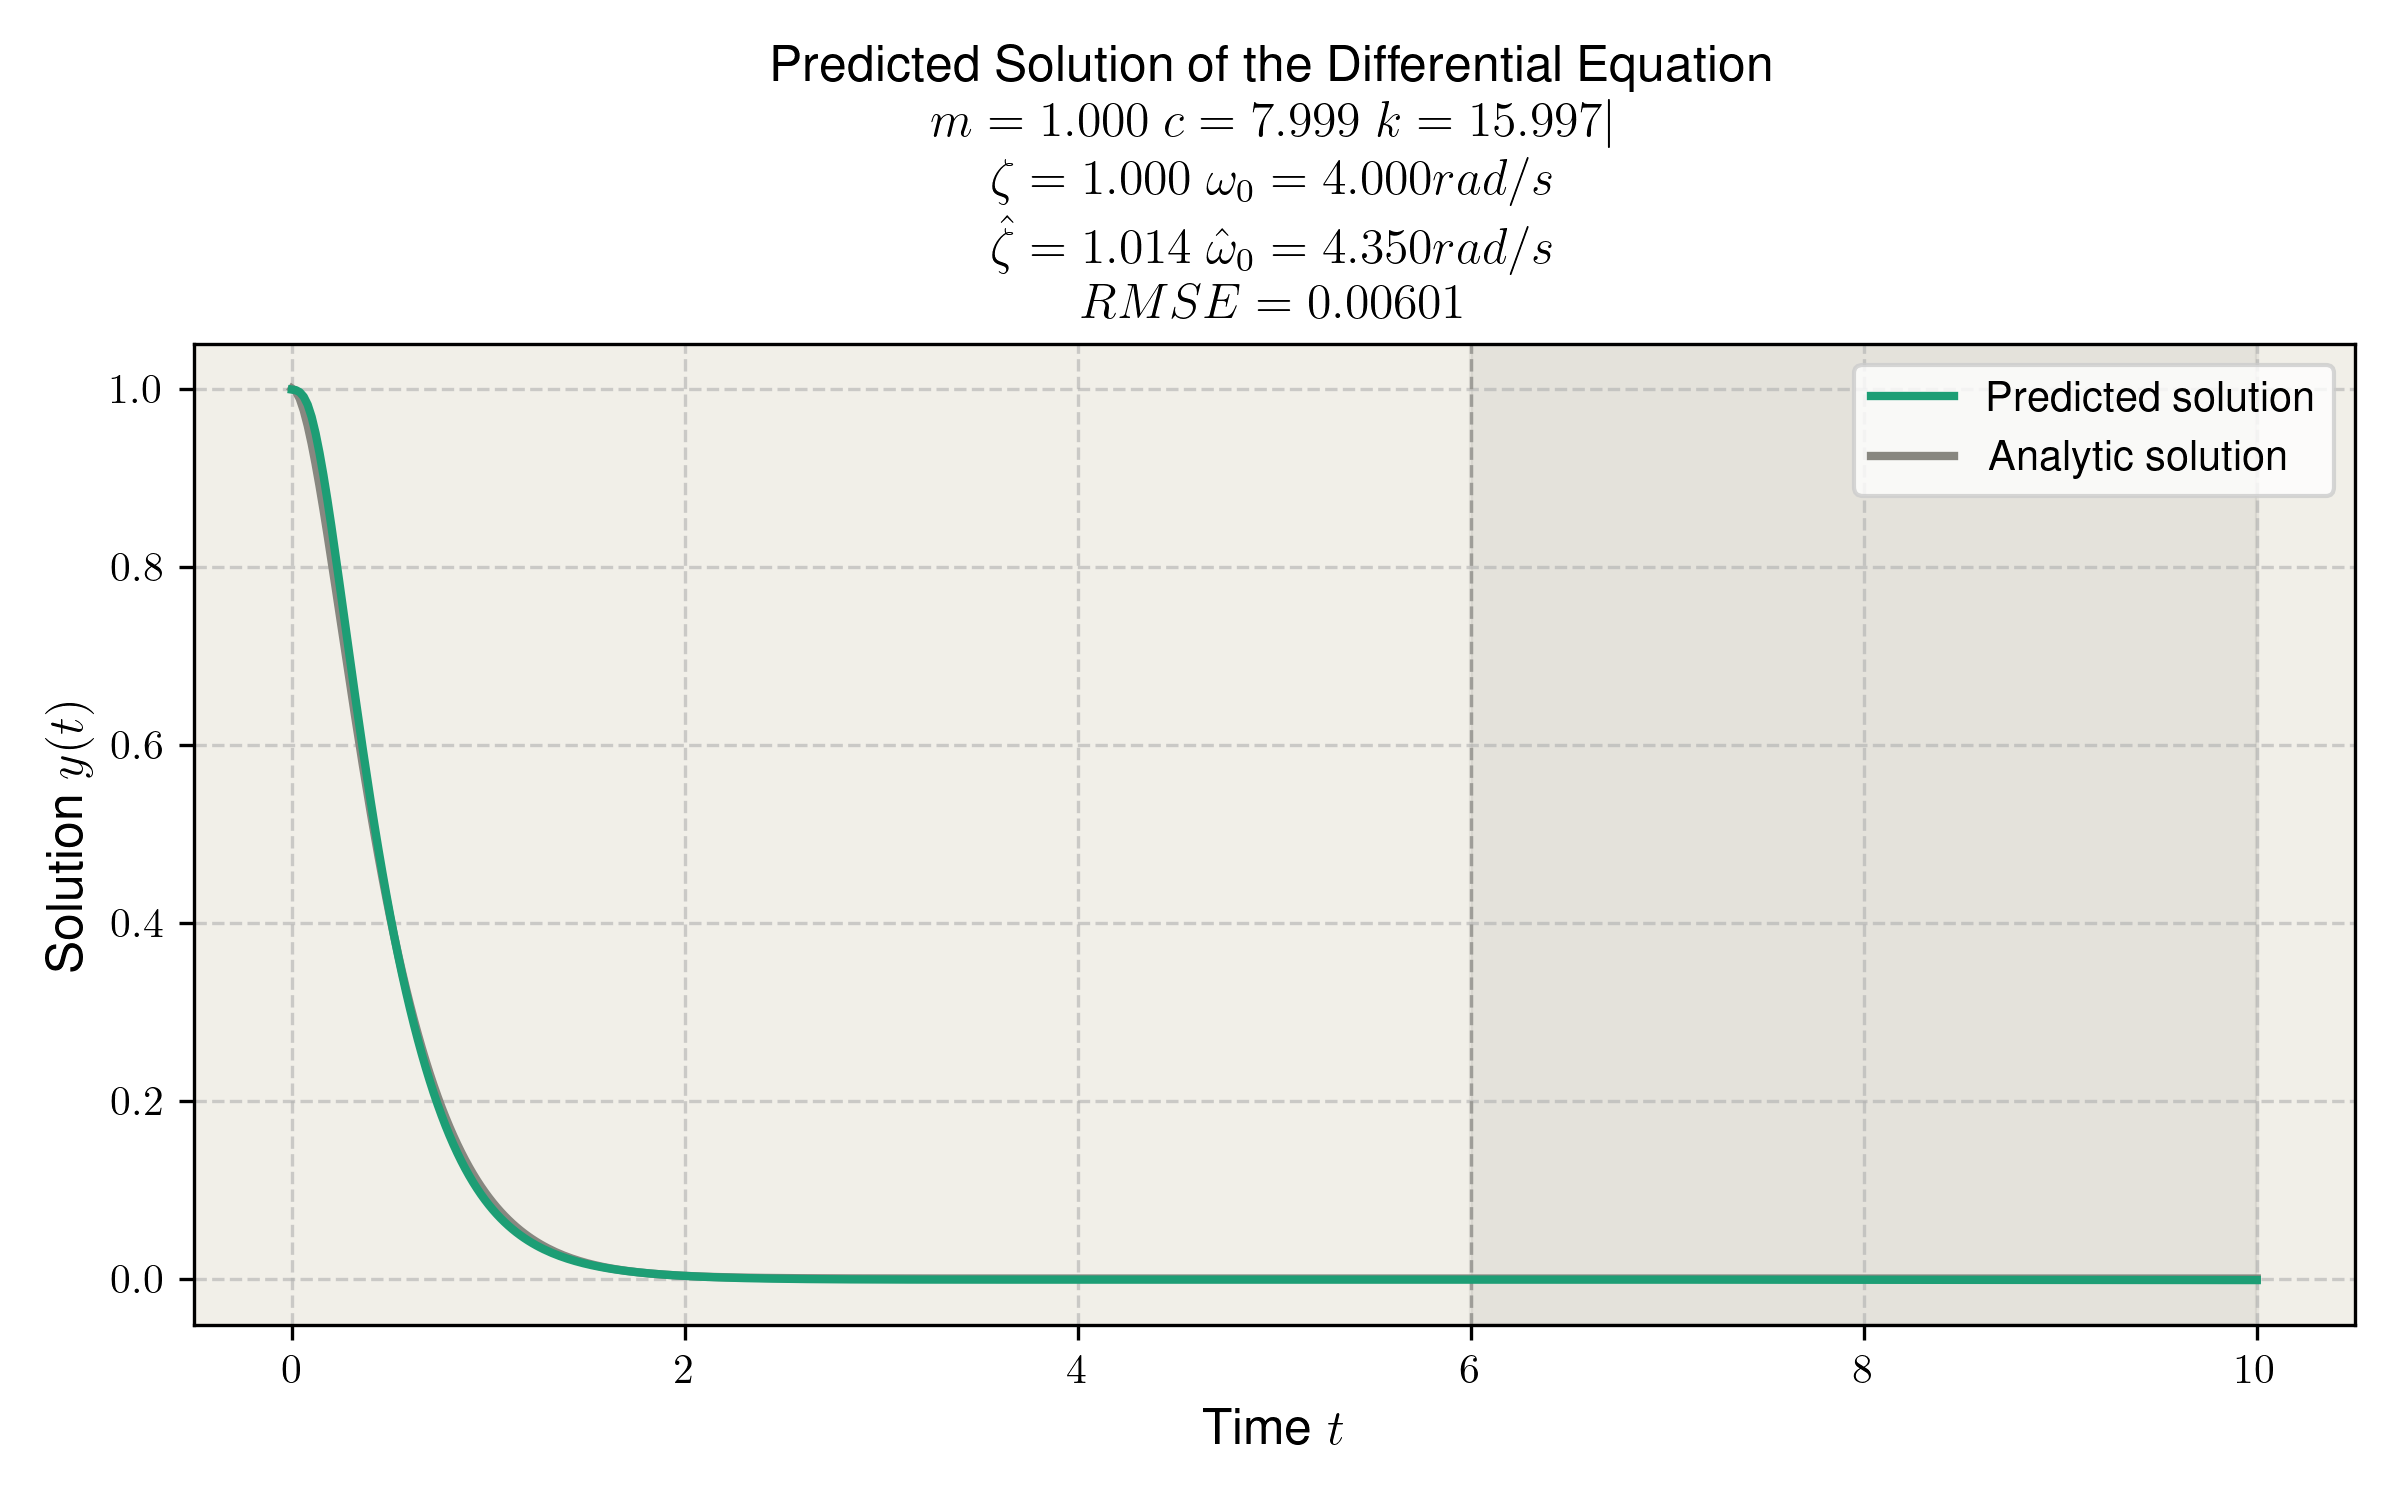
\includegraphics[width=0.75\textwidth]{Images_DHO/inversepinn_criticallydamped/predicted_solution.png}
    \caption{Predicted solution and parameters for a critically damped harmonic oscillator with randomised parameters.}
    \label{fig:inversepinn_criticallydamped/predicted_solution}
\end{figure}

\begin{figure}[H]
    \centering
    
\includegraphics[width=0.75\textwidth]{Images_DHO/inversepinn_criticallydamped/parameter_convergence.png}
    \caption{Parameter convergence to true values for a critically damped harmonic oscillator with randomised parameters.}
    \label{fig:inversepinn_criticallydamped/parameter_convergence}
\end{figure}
We can see that the model is able to recover the equation parameters with relatively good acuraccy for the critically damped case. Again, this case is very similar to the overdamped case so comparable results are expected.

\subsection{Underdamped case}
For the overdamped demonstration example, the randomised and predicted parameters are:
\begin{table}[H]
\centering
\caption{Overdamped parameters}
\begin{tabular}{lcc}
\toprule
\textbf{Parameter} & \textbf{True value} & \textbf{Predicted value} \\
\midrule
\texttt{$\zeta$}             & $0.160$ & $0.171$ \\
\texttt{$\omega_0$}          & $1.950$ & $1.961$   \\
\bottomrule
\end{tabular}
\end{table}

Figures \ref{fig:inversepinn_underdamped/predicted_solution} and \ref{fig:inversepinn_underdamped/parameter_convergence} show the predicted solution and parameter convergence to the true values.

\begin{figure}[H]
    \centering
    
\includegraphics[width=0.75\textwidth]{Images_DHO/inversepinn_underdamped/predicted_solution.png}
    \caption{Predicted solution and parameters for an underdamped harmonic oscillator with randomised parameters.}
    \label{fig:inversepinn_underdamped/predicted_solution}
\end{figure}

\begin{figure}[H]
    \centering
    
\includegraphics[width=0.75\textwidth]{Images_DHO/inversepinn_underdamped/parameter_convergence.png}
    \caption{Parameter convergence to true values for an underdamped harmonic oscillator with randomised parameters.}
    \label{fig:inversepinn_underdamped/parameter_convergence}
\end{figure}
We can see that the model is able to recover the equation parameters with great acuraccy for the underdamped case. The analytic solutions for this case are more dependent on the equation parameters than the previous two cases, so it is to be expected that the model can extract the parameters with the same or better acuraccy.

\subsection{Statistical analysis}\label{ch:stat_DHO}
This section is made using the \verb|inversepinn_data_generation.py| and \verb|inversepinn_plots.py| scripts. The previous three demonstration examples are a good illustration of the capabilities of the inverse model, but are not enough to make well-reasoned and statistically backed conlcusions about the model acuraccy. For this, we need a more quantifiable way to gauge the accuracy of the model.\\

One of the sources of uncertainty when estimating the parameters is the noise applied to the training observation points. The training points are randomised every epoch and should, in principle, not have much influence on the exact prediction, but it makes the process non-deterministic nonetheless. Furthermore, up until now we have only tested the parameter extraction on 3 $(\zeta,\ \omega_0)$ pairs. This is not yet representative for the model performance over a wide range of valeus for these parameters.\\

In order to account for both of these effects, we can run a large amount of parameter estimations with randomised equation parameters for every different model. This will both give an idea of the variance of the estimations due to the noisy training data, and generalise the three demonstration examples to a larger domain of $(\zeta,\ \omega_0)$ values. I have chosen to first randomize the damped case, with a $45\%$ chance of under- or overdamped and a $10\%$ chance of critically damped. Then, $(\zeta,\ \omega_0)$ is randomised and the inverse model is trained to estimate the parameters. In the end, $304$ total estimations were performed. Figures \ref{fig:parameter_estimation/scatter_zeta_full} and \ref{fig:parameter_estimation/scatter_omega_0_full} show the true-predicted parameter values.

\begin{figure}[H]
    \centering
    \begin{subfigure}[b]{0.48\textwidth}
        \centering
        
\includegraphics[width=\textwidth]{Images_DHO/parameter_estimation/scatter_zeta_full.png}
        \caption{Scatter plot of 304 true and predicted $\zeta$ pairs.}
        \label{fig:parameter_estimation/scatter_zeta_full}
    \end{subfigure}
    \hfill
    \begin{subfigure}[b]{0.48\textwidth}
        \centering
        
\includegraphics[width=\textwidth]{Images_DHO/parameter_estimation/scatter_omega_0_full.png}
        \caption{Scatter plot of 304 true and predicted $\omega_0$ pairs.}
        \label{fig:parameter_estimation/scatter_omega_0_full}
    \end{subfigure}
    \caption{Scatter plots of true and predicted physical parameters for the damped harmonic oscillator.}
    \label{fig:parameter_estimation/scatter_full}
\end{figure}

AS we can see, the estimations are quite good in general. For small parameter values, the model is very good at precisely extracting the true values. For larger values however, the model seems to underestimate the parameter values. To quantify this further, we can calulate the $RMSE$ of the two parameters in the three different cases. This leads to the following results:

\begin{table}[H]
\centering
\caption{Parameter estimation RMSE across different cases}
\begin{tabular}{lcc}
\toprule
\textbf{Case} & \textbf{RMSE $\zeta$} & \textbf{RMSE $\omega_0$} \\
\midrule
Full domain         & $0.1732$ & $0.4791$ \\
Underdamped         & $0.0351$ & $0.2960$ \\
Critically damped   & $0.0672$ & $0.4007$ \\
Overdamped          & $0.2649$ & $0.6415$ \\
\bottomrule
\end{tabular}
\end{table}

The $RSME$ indeed increases for the critically and overdamped cases. In order to also take the effect of $\omega_0$ into account, we can plot the \textit{parameter space}, where the axes represent $\zeta$ and $\omega_0$. Figure \ref{fig:parameter_estimation/scatter_omega_0_full} shows the $(\zeta,\ \omega_0)$ in the parameter space, color coded by the $RMSE$ of the predicted values.

\begin{figure}[H]
    \centering
    
\includegraphics[width=0.65\textwidth]{Images_DHO/parameter_estimation/parameter_space_rmse_full.png}
    \caption{Parameter space of 304 true $(\zeta, \omega_0)$ pairs and the $RMSE$ compared to the predicted values.}
    \label{fig:parameter_estimation/parameter_space_rmse_full}
\end{figure}

Again, we can see that large parameter values generally lead to a larger $RMSE$. One possible explanation is that the parameters become harder to extract because the soltuions to the ODE becone less and less dependent on the parameters. This is illustrated in the Figure \ref{fig:grid_zeta_omega}, where the solutions to the ODE are plotted for different values of $\zeta$ and $\omega_0$ in the underdamped and overdamped regime.

\begin{figure}[H]
    \centering
    \begin{subfigure}[b]{0.48\textwidth}
        \centering
        \includegraphics[width=\textwidth]{Images_DHO/analytic_solutions_zeta_underdamped.png}
        \caption{Underdamped solutions for different $\zeta$}
        \label{fig:analytic_solutions_zeta_underdamped}
    \end{subfigure}
    \hfill
    \begin{subfigure}[b]{0.48\textwidth}
        \centering
        \includegraphics[width=\textwidth]{Images_DHO/analytic_solutions_zeta_overdamped.png}
        \caption{Overdamped solutions for different $\zeta$}
        \label{fig:analytic_solutions_zeta_overdamped}
    \end{subfigure}

    \vspace{0.5em}

    \begin{subfigure}[b]{0.48\textwidth}
        \centering
        \includegraphics[width=\textwidth]{Images_DHO/analytic_solutions_omega_underdamped.png}
        \caption{Underdamped solutions for different $\omega_0$}
        \label{fig:analytic_solutions_omega_underdamped}
    \end{subfigure}
    \hfill
    \begin{subfigure}[b]{0.48\textwidth}
        \centering
        \includegraphics[width=\textwidth]{Images_DHO/analytic_solutions_omega_overdamped.png}
        \caption{Overdamped solutions for different $\omega_0$}
        \label{fig:analytic_solutions_omega_overdamped}
    \end{subfigure}

    \caption{}
    \label{fig:grid_zeta_omega}
\end{figure}

We can observe a lot more dispersion for the underdamped case, which means that the uncertainty of the estimates of the parameters will be smaller in this regime. For the overdamped case, the solutions are similar, and it is more difficult to extract the correct parameter value.\\

We can conclude that the most important source of uncertainty when estimating the equation parameters is the noise applied to the training data. We can investigate the uncertainty through a statistical approach where we estimate the parameters for a large amount of randomised equations, which also clarifies the model acuraccy in the different damped regimes. We conclude that the higher the damping, the more difficult the parameter extraction becomes since the solutions look very similar for variations in the parameters.

\chapter{Burger's Equation}
In this chapter, we will apply PINNs to solve the 1D Burger's equation, a PDE which describes convection and diffusion. The code for this chapter can be found in the \verb|Burgers_Equation| directory. The general form of the inviscid Burger's equation is given by:
\begin{equation}
    \frac{\partial u}{\partial t} + u\frac{\partial u}{\partial x}=0
\end{equation}
This equation is sometimes written in the following notation:
\begin{equation}
    u_t + uu_x = 0
\end{equation}
This is a hyperbolic first-orde PDE, which can be solved using the method of characteristics (see section\ref{ch:method_of_characteristics}).\\

This equation occurs in fluid dynamics, where the field $u(x,\ t)$ represents the velocity of the fluid. In our case, we are then studying a one-dimensional fluid. The term $u_t$ represents the rate of change in the velocity field. It is equal (if the viscosity is negligent) to the advection term $uu_x$, which gives a wave-like equation where the speed of the transported quantity $u$ is proportional to the value of $u$ itself \cite{vanremortel_einsle_2026}. This makes sense in the fluid dynamical interpretation of the equation; if interactions between the particles in the fluid can be ignored, and the velocity of each particle stays constant, the transport of the velocity is proportional to the velocity itself.\\

The fact that the transport speed scales with $u$ leads to interesting behavior. It means that the top of a wave will travel faster than the bottom of the wave, causing it to fold over on itself. This leads to the creation of a discontinuïty, which is called a \textit{shockwave}. On the other hand, when the gradient of $u$ is positive, it can lead to the top of a wave 'running away' from its base, leading to the velocity field being stretched out and the gradient decreasing. This is called a \textit{rarefaction}.\\

To avoid discontinuïties in the solution, which will lead to numerical instability, we can add a viscosity term $\nu\frac{\partial^2 u}{\partial x^2}$ which will prevent the formation of sharp gradients. In the fluid dynamical interpretation of the equation, this term represents the internal friction between the particles in the fluid. The viscid Burger's equation is given by:

\begin{equation}
    u_t + uu_x = \nu u_{xx}
\end{equation}

where $\nu$ iq called the \textit{kinematic viscosity}. This equation is now not hyperbolic, but parabolic. It cannot be solved using the method of characteristics and needs an initial condition $u(x,\ 0)$ and boundary conditions $u(0,\ t)$ and $u(L,\ t)$ to have a unique, well-defined solution. This is the equation we will attempt to solve using a PINN. 

\section{Ground truth solving strategies}
In order to train a machine learning model to solve the equation, we need ground truth data to use for the model training. Since we are not doing a real-world experiment, we do not have access to real data and have to simulate the ground truth data ourselves. In order to do this, there are multiple possible solving strategies.

\subsection{Method of characteristics}\label{ch:method_of_characteristics}
As explained before, the Method Of Characteristics (MOC) can only be used for the inviscid equation. MOC works by looking for $(x(s), t(s))$ curves along which teh PDE collapsed to an ODE for the parameter $s$. Consider such a curve, then the chain rule tells us that:
\begin{equation}
    \frac{du}{ds}=u_t\frac{dt}{ds} + u_x\frac{dx}{ds}
\end{equation}
Comparing this to the inviscid Burger's equation, we can equate the coefficients of $u_x$ and $u_t$:
\begin{equation}
    \begin{split}
        \frac{dt}{ds} =& 1 \rightarrow t=s\\
        \frac{dx}{ds} =& u \rightarrow \frac{dx}{dt} = u\\
        \frac{du}{ds} =& 0 \rightarrow u(s) = u_0(x)
    \end{split}
\end{equation}

This implies that the solution $u$ remains constant along curves $x(t)=u_0(x)t+x_0$. This can be used to solve the equation, as shown on Figures \ref{fig:gauss_characteristics} and \ref{fig:gauss_ic_t}.

\begin{figure}[H]
    \centering
    \includegraphics[width=0.9\textwidth]{Images_DHO/gauss_characteristics.png}
    \caption{Method of characteristics applied to a Gaussian initial condition.}
    \label{fig:gauss_characteristics}
\end{figure}


\begin{figure}[H]
    \centering
    \begin{subfigure}[b]{0.48\textwidth}
        \centering
        \includegraphics[width=\textwidth]{Images_DHO/gauss_ic.png}
        \caption{Initial Gauss condition.}
        \label{fig:gauss_ic}
    \end{subfigure}
    \hfill
    \begin{subfigure}[b]{0.48\textwidth}
        \centering
        \includegraphics[width=\textwidth]{Images_DHO/gauss_t.png}
        \caption{Gauss at $t=1$.}
        \label{fig:gauss_t}
    \end{subfigure}
    \caption{Gaussian initial condition and its time evolution.}
    \label{fig:gauss_ic_t}
\end{figure}

This is a powerful method to predict when a shock will occur; a shockwave takes place when two characteristics cross, which is equal to $t = -\frac{1}{\min_x u_x(x,\ t=0)}$. This \textit{shock time} is also indicated on Figure \ref{fig:gauss_characteristics}. However, we will be concerned with the viscid equation when training a PINN. To get ground truth solutions, we must look at other solving algorithms which are also capable of solving the viscid equation.

\subsection{Numerical PDE solvers}
The first option is to implement numerical iterative methods, which use finite-differences to discretize the derivatives in the equation. The solution is then calculated by dividing the releavnt domain into a grid with spacings $\Delta x$ and $\Delta t$, and continously solving for the soltuion at the next $\Delta t$. I implemented two different discretisation schemes:

\subsubsection{Euler's method (upwind)}
Using Euler's method with upwind advection, the scheme is first order in time and first order in space for the advection term. The diffusion term is handled  with second-order central differences. The discretisation scheme becomes:

\begin{equation}
    u_i^{n+1} = u_i^n - \Delta t \ A_i^n + \Delta t \ \nu \frac{u_{i+1}^n - 2u_i^n + u_{i-1}^n}{\Delta x^2}
\end{equation}

where the upwind advection term $A_i^n$ is chosen based on the sign of $u_i^n$:

\begin{equation}
    A_i^n = \begin{cases}
        u_i^n \dfrac{u_i^n - u_{i-1}^n}{\Delta x} & \text{if } u_i^n \geq 0 \quad \text{(backward difference)} \\[10pt]
        u_i^n \dfrac{u_{i+1}^n - u_i^n}{\Delta x} & \text{if } u_i^n < 0 \quad \text{(forward difference)}
    \end{cases}
\end{equation}

The upwind scheme selects the finite difference direction based on the local flow direction, which improves numerical stability by respecting the characteristic direction of the advection term.

\subsubsection{Lax-Wendroff scheme}
Using the Lax-Wendroff scheme, which is second order in both time and space (both diffusion and advection), the discretisation scheme becomes:

\begin{equation}
    u_i^{n+1} = u_i^n - \frac{\Delta t}{\Delta x}\left(F_{i+\frac{1}{2}}^n - F_{i-\frac{1}{2}}^n\right) + \Delta t \ \nu \frac{u_{i+1}^n - 2u_i^n + u_{i-1}^n}{\Delta x^2}
\end{equation}

with the Burgers flux $f_i^n = \tfrac{1}{2}(u_i^n)^2$ and local wave speed $c_{i+\frac{1}{2}}^n = \tfrac{1}{2}(u_i^n + u_{i+1}^n)$. The diffusion term is handled separately with second-order central differences. The Lax-Wendroff scheme reduces numerical diffusion compared to the upwind Euler method, at the cost of introducing small oscillations near sharp gradients.\\

Numerical schemes can be a powerful method to calculate the ground truth, but we have no good way of validating the accuracy of the result.  Numerical errors will propagate and increase with time, depending on the accuracy of the discretisation scheme. Calculating the physics residual using finite differences would be a circular reasoning, since the solutions were constructed using the very same discretisation; we would simply be reversing the calculations that have alreade been done, which gives a very low residual. This means that it is difficult to be sure of the accuracy of the ground truth. Therefore, I have chosen a different methodology.

\subsection{Cole-Hopf Transformation}
The viscid Burger's equation can be solved by applying the \textit{Cole-Hopf Transformation}:
\begin{equation}
    u = -2\nu \frac{\phi_x}{\phi}
\end{equation}
Through a lengthy calculation \cite{whitham2011linear}, we find that the Burger's equation is transformed into the heat equation:
\begin{equation}
    \phi_t = \nu\phi_{xx}
\end{equation}
This equation has a closed-form solution once the initial condition $\phi(x,t=0)=\phi_0(x)$ is defined by convoluting with the heat kernel:
\begin{equation}
    \phi(x,t)
    =
    \frac{1}{\sqrt{4\pi \nu t}}
    \int_{-\infty}^{\infty}
    \phi_0(x')
    \exp\left(
        -\frac{(x-x')^2}{4\nu t}
    \right)\,dx'.
\end{equation}
With this solution, we can recover $u(x,\ t)$ for ant value of $t$. For some initial conditions, analytic solutions to the Burger's equation can be found using this method. For more flexibility, I have chosen to solve the convolution integral numerically, so that any initial condition can be used as a ground truth.\\

It is obviously impossible to evaluate the convolution integral from $-\infty$ to $+\infty$ numerically. However, if we constrain the domain of the integral to $[0,\, L]$ where $L$ is the length of our system, boundary effects will occur since the heat kernel will be cut off at the edges. To fix this, we pad the sides of the initial condition with a constant function matching the Dirichlet boundary condition so the domain is extrapolated. We then compute the ground truth solution using the Carl-Hopf method, and remove the paddings. In this way, we can also apply Dirichlet boundary conditions at a finite interval.\\

For validation, it is wise to calculate the $RMSE$ of the physics residual. For a gaussian initial condition with $\nu=0.01$ and $t_{end}=10$, this yields:
\begin{equation*}
    RMSE=5.19\cdot 10^{-6}
\end{equation*}
This is a very small residual, which confirms the transformation can give us accurate solutions of the Burger's equation.\\

Using this method, I calculate the values for $u(x,\ t)$ on a dense grid of points. In order to randomise the data generation even more and avoid fine tuning to the specific spacings of this grid, I will make noisy data points by making a bilinear interpolation of the ground truth solution grid.
\section{PINNs for the Burger's equation}
With the ground truth data simulation method chosen, we can now train PINNs to solve the viscid Burger's equation. Just like for the damped harmonic oscillator, I will discuss the code implementation and show some examples, study the different loss terms and hyperparameters, and finally attempt to solve the inverse problem.\\

The implementation of the neural network is strongly based on the implementation of the damped harmonic oscillator PINN. The same improvements I have previously discussed apply; randomised training data and collocation points, early stopping, and model saving have all been implemented. The most important change is obviously the model itself, which now takes two inputs $(x, t)$ instead of one input $(t)$. This means that the loss functions and plotting methods also need to be adapted to handle two dimensional data.\\

Furthermore, we are instructed to not give the model any training observations when solving the PDE in the first part of this task; data points can only be added in the second part where we need to extract $\nu$. It is obviously not possible to extract equation parameters without data points. In order to implement this, I have defined a new parameter \verb|use_data| in the \verb|Config| class, which acts as a switch for adding data points to the training loop. In the first part of this exercise, the variable will be set to False.\\

Some more adaptations that require an bit more in-depth explanation are included below.
\subsection{File structure}
The structure of the code is roughly the same as for the damped harmonic oscillator:
\begin{tcolorbox}[title=Burger's equation file structure, colback=black!10!white, colframe=black!40!white, sharp corners]
\begin{verbatim}
Burgers_Equation/
|-- config.py           - dataclass holding all physical constants,
|                        hyperparameters, runtime settings
|-- analytic.py          - ground truth solution schemes, including
|                        upwind euler, lax-wendroff and Cole-Hopf method
|-- data.py             - data generation based on ground truth solutions
|                        for collocation points, observation points,
|                        and initial conditions
|-- model.py            - FCNet architecture and predictor functions
|-- losses.py           - loss functions for the training of the model
|-- trainer.py          - training loop
|-- plot.py             - all plotting functions
|-- utils.py            - helper file for small functions
\end{verbatim}
\end{tcolorbox}
The only notable difference compared to the damped harmonic oscillator is the inclusion of the \verb|analytic.py| file. The ground truth is now much more complex to calculate than for the damped harmonic oscillator, so I have chosen to do all the ground truth solution generation in a separate file. 
\subsection{Boundary condition loss}
We introduce a new loss term: $\mathcal{L}_{b.c.}$ to force the PINN to respect the boundary conditions of the system. Every epoch, 50 boundary condition points are chosen randomly along both boundaries of the system (at $x=0$ and $x=L$) and the predicted value $\hat y$ and derivative $d\hat y$ are evaluated (using \verb|autograd|). The loss term $\mathcal{L}_{b.c.}$ and total loss are then calculated as:
\begin{equation}
    \begin{split}
        \mathcal{L}_{b.c.} &= \frac{1}{N}\sum^N_{i=1}\left[(y_{i,\ left}-\hat y_{i,\ left})^2 + (y_{i,\ right}-\hat y_{i,\ right})^2\right]\\
        \mathcal{L}_{tot} &= \lambda_{i.c.}\mathcal{L}_{i.c.} + \lambda_{b.c.}\mathcal{L}_{b.c.} + \lambda_{phys}\mathcal{L}_{phys}
    \end{split}
\end{equation}
\subsection{Plotting methods}
I have implemented a wide range of plotting methods, which are described below.  I have used the Sonnet 4.6 model from Claude AI to assist me with the design of these plots. 
\begin{itemize}
    \item A plot of the characteristics of the inviscid equation and the predicted shock time $t_{shock}$.
    \item A plot of the ground truth solution calculated using the Cole-Hopf transformation at four different times ($t=0,\ t=2,\ t=4,\ t=6$).
    \item A plot of the ground truth and predicted solution at four different times ($t=0,\ t=2,\ t=4,\ t=6$).
    \item A plot of the ground truth and predicted solution at eoght different, evenly spaced times from $t=0$ to $t=t_{extrap}$.
    \item A plot of the ground truth and predicted solution at three different times ($t=0,\ t=t_{shock}/2,\ t=t_{shock}$)\footnote{This is the plot that is explictly requested in the assignment.}.
    \item A 2D plot of the full ground truth solution (displayed as a matrix).
    \item A 2D plot of the full predicted solution (displayed as a matrix).
    \item A plot of the different loss terms as a funtion of the epochs.
    \item A plot with 6 subplots showing the convergence of the predicted solution as a function of the epochs.
    \item A summary plot with 6 panels containing the following:
    \begin{enumerate}
        \item A 2D plot of the full ground truth solution.
        \item A 2D plot of the full predicted solution.
        \item A 2D plot of the square of the physics residual $|u_t+uu_x-\nu uu_{xx}|^2$.
        \item A 3D surface plot of the predicted solution.
        \item A plot of the different loss terms as a funtion of the epochs.
        \item A 2D plot of the validation MSE $|\hat u(x, t)-u(x, t)|^2$
    \end{enumerate}
\end{itemize}
An example of every plot will be shown in section \ref{ch:gauss}.
\section{Code demonstration}
This section is made using the \verb|pinn_demo.py| script\footnote{And also the pinn\_cases.py script for automisation}. In this section, we will demonstrate PINNs for three different initial conditions (Gauss, N-wave and Step-up functions), and three different values for the viscosity ($\nu=0.1,\ 0.05,\ 0.01$). Unless specified otherwise, we will use the following hyperparameters:

\begin{table}[H]
\centering
\caption{PINN Hyperparameters}\label{tab:standard_parameters_BE}
\begin{tabular}{llc}
\toprule
\textbf{Parameter} & \textbf{Description} & \textbf{Value} \\
\midrule
\texttt{hidden}               & Hidden units per layer            & 96                   \\
\texttt{n\_layers}            & Number of hidden layers           & 8                    \\
\texttt{n\_epochs}            & Maximum training epochs           & 30000                \\
\texttt{lr}                   & Initial learning rate             & $2\times10^{-3}$     \\
\texttt{patience}             & Early stopping patience           & 5000                 \\
\texttt{patience\_threshold}  & Min improvement to reset patience & $2\times10^{-6}$     \\
\texttt{scheduler\_step}      & LR scheduler step size            & 3000                 \\
\texttt{scheduler\_gamma}     & LR scheduler decay factor         & $0.5$                \\
\texttt{lambda\_phys}         & Physics loss weight               & $5$                  \\
\texttt{lambda\_ic}           & Initial condition loss weight     & $1\times10^{1}$      \\
\texttt{lambda\_bc}           & Boundary condition loss weight    & $1\times10^{1}$      \\
\texttt{n\_col\_dom}          & Collocation points                & 200                  \\
\texttt{n\_bc}                & Boundary condition points         & 50                   \\
\bottomrule
\end{tabular}
\end{table}
Just like before, these hyperparameters have been hand-picked and are observed to give reasonable results. We will tune the hyperparameters (with inclusion of observation points) in section \ref{ch:hyperparameters_BE}.

\subsection{Gauss}\label{ch:gauss}
The gauss initial condition is given by:
\begin{equation}
    u(x,\ t=0) = A\exp\left[-\frac{\left(x-\frac{L}{2}\right)^2}{2\sigma^2}\right]
\end{equation}
In this case, we have chosen $L=15,\ \sigma=1 ,\ A=0.7$ Through the method of characteristics, we can predict the time when a shockwave will form by approximating the solution by the inviscid case. This yelds $t_{shock}=2.353$. The method of characteristics is shown on Figure  
\begin{figure}[H]
    \centering
    
\includegraphics[width=0.65\textwidth]{Images_BE/Gauss_nu_0.1/method_of_characteristics.png}
    \caption{Method of characteristics applied to a Gaussian initial condition.}
    \label{fig:Gauss_nu_0.1/method_of_characteristics}
\end{figure}
We will now train PINNs to predict the solution to the equation for three different values for $\nu$. In the next sections, I will discuss these results.\\

\subsubsection{Gauss, $\nu=0.05$}
To begin, we choose $\nu=0.05$. This is a good strating value, since it is not too high or too low. The ground truth solution calculated by the Cole-Hopf transformation is shown on Figure \ref{fig:Gauss_nu_0.05_gt}.
\begin{figure}[H]
    \centering
    \begin{subfigure}[b]{0.58\textwidth}
        \centering
        
\includegraphics[width=\textwidth]{Images_BE/Gauss_nu_0.05/gt_solution.png}
        \caption{3D solution.}
        \label{fig:Gauss_nu_0.05_gt_solution}
    \end{subfigure}
    \hfill
    \begin{subfigure}[b]{0.4\textwidth}
        \centering
        
\includegraphics[width=\textwidth]{Images_BE/Gauss_nu_0.05/gt_2D.png}
        \caption{2D solution.}
        \label{fig:Gauss_nu_0.05_gt_2D}
    \end{subfigure}
    \caption{Ground truth solution to the gaussian initial conditions calculated witht eh Cole-Hopf transformation.}
    \label{fig:Gauss_nu_0.05_gt}
\end{figure}
We can indeed observe the formation of a shock front in the ground truth solution. The gaussian wave tilts to the right, which creates a steep gradient. A more or less stationary configuration is reached when the gradient becomes so steep that viscosity term becomes so large that it prevents the gradient from becoming even steeper.\\

On the 2D-plot, we can see that the viscous term causes the shockwave to occur later than the predicted time. In fact, a shockwave in its most formal definition is never formed, since the viscous term prevents the formation of discontinuïties. When we talk about a shockwave in this context, we are referring to the point where the gradiënt becomes so steep that the viscous term has slowed down the propagation of the field to a relatively stationary regime.\\

The PINN is now trained, and the predicted solution at the three requested valeus for $t$ (initial condition, before shock and after shock) are shown on Figure \ref{fig:Gauss_nu_0.05/3_times}. The training is stopped early after $9450$ epochs and the final $RMSE$ is $RMSE=0.0052$. From these results, we can see that the model is able to fit to the ground truth to a gaussian initial condition with this viscosity solution very accurately. For this case, I will also demonstrate all the other plotting methods that I have implemented in the code. Figures \ref{fig:Gauss_nu_0.05/gt_2D} and \ref{fig:Gauss_nu_0.05/pred_2D} show the analytic and predicted solutions plotted as 2D matrices.

\begin{figure}[H]
    \centering
    
\includegraphics[width=0.8\textwidth]{Images_BE/Gauss_nu_0.05/3_times.png}
    \caption{Predicted solutions at start time, before shock time and at shock time for gaussian initial conditions and $\nu=0.05$.}
    \label{fig:Gauss_nu_0.05/3_times}
\end{figure}

\begin{figure}[H]
    \centering
    \begin{subfigure}{0.48\textwidth}
        \centering
        
\includegraphics[width=\textwidth]{Images_BE/Gauss_nu_0.05/gt_2D.png}
        \caption{Ground truth solution in 2D for gaussian initial conditions and $\nu=0.05$.}
        \label{fig:Gauss_nu_0.05/gt_2D}
    \end{subfigure}
    \hfill
    \begin{subfigure}{0.48\textwidth}
        \centering
        
\includegraphics[width=\textwidth]{Images_BE/Gauss_nu_0.05/pred_2D.png}
        \caption{Predicted solutions in 2D for gaussian initial conditions and $\nu=0.05$.}
        \label{fig:Gauss_nu_0.05/pred_2D}
    \end{subfigure}
    \caption{Ground truth and predicted solutions in 2D for gaussian initial conditions and $\nu=0.05$.}
    \label{fig:Gauss_nu_0.05_2D}
\end{figure}

We again see a very good agreement between the prediction and true solution. These plots are useful because they give a full overview of the solution, something which is not possible when plotting slices of the solution $u(x,\ t)$ with constant $t$ like in Figure \ref{fig:Gauss_nu_0.05/3_times}. However, it is more difficult to spot small deviations form the ground truth solution since the solutions cannot directly be compared like in Figure \ref{fig:Gauss_nu_0.05/3_times}. Both plotting the entire solution as a 2D image, and plotting mutple time slices at discrete times have their advantages and disadvantages. Figures \ref{fig:Gauss_nu_0.05/pred_solution} and \ref{fig:Gauss_nu_0.05/pred_grid} show the predicted solution at more values for $t$.

\begin{figure}[H]
    \centering
    
\includegraphics[width=0.8\textwidth]{Images_BE/Gauss_nu_0.05/pred_solution.png}
    \caption{Predicted solutions at 8 different times for gaussian initial conditions and $\nu=0.05$.}
    \label{fig:Gauss_nu_0.05/pred_solution}
\end{figure}

\begin{figure}[H]
    \centering
    
\includegraphics[width=0.8\textwidth]{Images_BE/Gauss_nu_0.05/pred_grid.png}
    \caption{Predicted solutions at 8 different times for gaussian initial conditions and $\nu=0.05$.}
    \label{fig:Gauss_nu_0.05/pred_grid}
\end{figure}

I have chosen to implement these plots since they can be useful in cases where the predicted solution deviates strongly from the ground truth solution. The network can usually fit to the initial condition accurately, after which more errors can start to occur for larger and larger values of $t$. Plotting the solution at many different times can then help to pinpoint where the solution starts to deviate strongly, and what exactly is going wrong. In this case, the predicted solution is very accurate so not a lot of additional information can be extracted by these plots. Figure \ref{fig:Gauss_nu_0.05/losses} shows the losses as a function of the epochs.

\begin{figure}[H]
    \centering
    
\includegraphics[width=0.65\textwidth]{Images_BE/Gauss_nu_0.05/losses.png}
    \caption{Convergence of loss function terms for gaussian initial conditions and $\nu=0.05$.}
    \label{fig:Gauss_nu_0.05/losses}
\end{figure}

The loss plot is usefull to see which contributions to the loss functions are the greatest, and to pinpoint when the model starts to overfit. $\mathcal{L}_{b.c.}$ and $\mathcal{L}_{b.c.}$ decrease the fastest, since they are the largest contributions to the total loss function and largely determine the optimisation of the parameters in the early stages of training. interestingly, the physics and validation loss functions show a large jump around $8000$ epochs. After this, the solution never reaches the lowest validation loss again and the training is stopped early. Since the validation loss is not decreasing fast enough, this is an indication that the learning rate or patience might have to be increased. Hovewer, the final solution is still very accurate, so this is a only a minor problem. Figure \ref{fig:Gauss_nu_0.05/losses} is a summary plot with the most important information about the prediction.

\begin{figure}[H]
    \centering
    
\includegraphics[width=0.8\textwidth]{Images_BE/Gauss_nu_0.05/summary.png}
    \caption{Summary plot for the predicted solution by a PINN for gaussian initial conditions and $\nu=0.05$.}
    \label{fig:Gauss_nu_0.05/summary}
\end{figure}

This plot gives a good general overview of the model performance. When looking at the 2D residual plots, we can observe that the error is the largest where the gradient of the solution is the largest. This makes sense, as the model uses a smooth activation funtion ($\tanh$) which makes it 'unnatural' to represent very sharp features; it will then also have the most trouble fitting to there regions. The final residual is hovewer still small, and the model performance is generally good.\\

To avoid this report from becoming too long, I will not show all generated plots for each and every case. For the rest of the demonstration cases, I will only show a plot of the rpedicted solution at different times, and the summary plot. They should give a good general idea of the model performance, but all generated plots can be found in the \verb|Burgers_Equation/outputs| directory.
\clearpage

\subsubsection{Gauss, $\nu=0.1$}
Let us now see what happens if the viscosity is increased to $\nu=0.1$. This results the prediction shown on Figures \ref{fig:Gauss_nu_0.1/3_times} and \ref{fig:Gauss_nu_0.1/summary}. A solution is reached after $6050$ epochs and the final $RMSE$ is $RMSE=0.0025$. The model is able to predict the solution with a higher viscosity with an even better accuracy, and the results look very similar to the results with $\nu=0.05$. This is not surprising as the ground truth solution actually looks pretty similar to the previous case; the higher viscosity just prevents the formation of an even steeper gradient, which is exactly what the model struggles to predict. A higher viscosity actually makes the solution easier to predict.
\begin{figure}[H]
    \centering
    
\includegraphics[width=0.4\textwidth]{Images_BE/Gauss_nu_0.1/3_times.png}
    \caption{Predicted solutions at start time, before shock time and at shock time for gaussian initial conditions and $\nu=0.1$.}
    \label{fig:Gauss_nu_0.1/3_times}
\end{figure}

\begin{figure}[H]
    \centering
    
\includegraphics[width=0.6\textwidth]{Images_BE/Gauss_nu_0.1/summary.png}
    \caption{Summary plot for the predicted solution by a PINN for gaussian initial conditions and $\nu=0.1$.}
    \label{fig:Gauss_nu_0.1/summary}
\end{figure}

\subsubsection{Gauss, $\nu=0.01$}
Let us now see what happens if the viscosity is decreased to $\nu=0.01$. This results in the following prediction:
\begin{figure}[H]
    \centering
    
\includegraphics[width=0.45\textwidth]{Images_BE/Gauss_nu_0.01_bad/3_times.png}
    \caption{Predicted solutions at start time, before shock time and at shock time for gaussian initial conditions and $\nu=0.01$.}
    \label{fig:Gauss_nu_0.01/3_times_bad}
\end{figure}

\begin{figure}[H]
    \centering
    
\includegraphics[width=0.7\textwidth]{Images_BE/Gauss_nu_0.01/summary.png}
    \caption{Summary plot for the predicted solution by a PINN for gaussian initial conditions and $\nu=0.01$.}
    \label{fig:Gauss_nu_0.01/summary_bad}
\end{figure}

As we can see, the model fails to predict the correct solution. It seems that the steeper gradient prevents the model from fitting accurately to the ground truth solution. To get a better result, the hyperparameters need to be tweaked. I have decided to increase the number of layers from 8 to 10, decrease the learning rate to $1\cdot 10^{-3}$, and increase the physics loss weight to $5$. The solution then converges after $11167$ epochs with a final $RMSE$ of $RMSE=0.0064$

\begin{figure}[H]
    \centering
    
\includegraphics[width=0.4\textwidth]{Images_BE/Gauss_nu_0.01/3_times.png}
    \caption{Predicted solutions at start time, before shock time and at shock time for gaussian initial conditions and $\nu=0.01$.}
    \label{fig:Gauss_nu_0.01/3_times}
\end{figure}

\begin{figure}[H]
    \centering
    
\includegraphics[width=0.7\textwidth]{Images_BE/Gauss_nu_0.01/summary.png}
    \caption{Summary plot for the predicted solution by a PINN for gaussian initial conditions and $\nu=0.01$.}
    \label{fig:Gauss_nu_0.01/summary}
\end{figure}
This now gives better results. The model complexity had to be increased for the model to be able to learn the steep gradient. This will be discussed in more detail in section \ref{ch:complexity_BE}.

\subsection{N-wave}
The N-wave initial condition is given by:
\begin{equation}
    u(x,\ t=0) = 
    \begin{cases}
        0 & \text{if} |x| > w\\
        -Ax & \text{if} |x| \leq w
    \end{cases}
\end{equation}
Where $w$ is the width of the wave and $A$ is the height of the wave. In this case, we have chosen $L=15, \ w=3, \ A=\frac{1}{3}$. Just like with the gaussian initial conditions, we can predict the time when a shockwave will form by approximating the solution by the inviscid case. This yelds $t_{shock}=3.000$. The method of characteristics is shown on Figure \ref{fig:N_wave_nu_0.05_bad/method_of_characteristics}.
\begin{figure}[H]
    \centering
    
\includegraphics[width=0.65\textwidth]{Images_BE/N_wave_nu_0.05_bad/method_of_characteristics.png}
    \caption{Method of characteristics applied to an N-wave initial condition.}
    \label{fig:N_wave_nu_0.1/method_of_characteristics}
\end{figure}
At $t=3$, many characteristics cross and a large shockwave is formed in the middle of the domain. We will now solve the equation for three different values for $\nu$, in the same way as for the gaussian initial conditions.
\subsubsection{N-wave, $\nu=0.05$}
For a normal value for the viscosity, the prediction gives the following output:
\begin{figure}[H]
    \centering
    
\includegraphics[width=0.5\textwidth]{Images_BE/N_wave_nu_0.05_bad/3_times.png}
    \caption{Predicted solutions at start time, before shock time and at shock time for N-wave initial conditions and $\nu=0.05$.}
    \label{fig:N_wave_nu_0.05_bad/3_times}
\end{figure}

\begin{figure}[H]
    \centering
    
\includegraphics[width=0.8\textwidth]{Images_BE/N_wave_nu_0.05_bad/summary.png}
    \caption{Summary plot for the predicted solution by a PINN for N-wave initial conditions and $\nu=0.05$.}
    \label{fig:N_wave_nu_0.05_bad/summary}
\end{figure}

We can see that the model has a lot of trouble fitting to predicted solution, and is not capable of replicating the discontinuities the initial conditions. Since the entire solution is based on these initial conditions, the result is not very accurate. To fix this, we can use the ground truth solution at a later time as the inital conditions, since the viscosity term will have smoothened out the discontinuities. I have chosen to start the predictions at $t=0.5$. This results in the following predictions, where the solution converges after 7750 epochs and the final $RMSE$ is $RMSE=0.0017$

\begin{figure}[H]
    \centering
    
\includegraphics[width=0.4\textwidth]{Images_BE/N_wave_nu_0.05/3_times.png}
    \caption{Predicted solutions at start time, before shock time and at shock time for N-wave initial conditions and $\nu=0.05$.}
    \label{fig:N_wave_nu_0.05/3_times}
\end{figure}

\begin{figure}[H]
    \centering
    
\includegraphics[width=0.7\textwidth]{Images_BE/N_wave_nu_0.05/summary.png}
    \caption{Summary plot for the predicted solution by a PINN for N-wave initial conditions and $\nu=0.05$.}
    \label{fig:N_wave_nu_0.05/summary}
\end{figure}
\clearpage
\subsubsection{N-wave, $\nu=0.1$}
Let us now see what happens if the viscosity is increased to $\nu=0.1$. This results in the following predictions, where the solution converges after 5800 epochs and the final $RMSE$ is $RMSE=0.0027$
\begin{figure}[H]
    \centering
    
\includegraphics[width=0.45\textwidth]{Images_BE/N_wave_nu_0.1/3_times.png}
    \caption{Predicted solutions at start time, before shock time and at shock time for N-wave initial conditions and $\nu=0.1$.}
    \label{fig:N_wave_nu_0.1/3_times}
\end{figure}

\begin{figure}[H]
    \centering
    
\includegraphics[width=0.7\textwidth]{Images_BE/N_wave_nu_0.1/summary.png}
    \caption{Summary plot for the predicted solution by a PINN for N-wave initial conditions and $\nu=0.1$.}
    \label{fig:N_wave_nu_0.1/summary}
\end{figure}
\clearpage
\subsubsection{N-wave, $\nu=0.01$}
Let us now see what happens if the viscosity is decreased to $\nu=0.01$. This results in the following predictions, where the solution converges after 8800 epochs and the final $RMSE$ is $RMSE=0.0696$
\begin{figure}[H]
    \centering
    
\includegraphics[width=0.4\textwidth]{Images_BE/N_wave_nu_0.01/3_times.png}
    \caption{Predicted solutions at start time, before shock time and at shock time for N-wave initial conditions and $\nu=0.01$.}
    \label{fig:N_wave_nu_0.01/3_times}
\end{figure}

\begin{figure}[H]
    \centering
    
\includegraphics[width=0.7\textwidth]{Images_BE/N_wave_nu_0.01/summary.png}
    \caption{Summary plot for the predicted solution by a PINN for N-wave initial conditions and $\nu=0.01$.}
    \label{fig:N_wave_nu_0.01/summary}
\end{figure}

It seems even with the smoothened initial conditions, the PINN is having trouble solving the PDE for low viscosities. Likely the derivatives of the solution are too sharp for the dense network with $\tanh$ activation funtions to generate gradients steep enough to find the actual soltuion.

\subsection{Step-up}
The Step-up initial condition is given by:
\begin{equation}
    u(x,\ t=0) = 
    \begin{cases}
        0 & \text{if} x < \frac{L}{2}\\
        A & \text{if} x > \frac{L}{2}
    \end{cases}
\end{equation}
Where $A$ is the height of the step function. In this case, we have chosen $L=15, \ A=1$. This solution does not produce a shockwave, since the gradient is positive everywhere. The characteristics do not cross, as shown on Figure \ref{fig:Step_up_nu_0.1/method_of_characteristics}.
\begin{figure}[H]
    \centering
    
\includegraphics[width=0.65\textwidth]{Images_BE/Step_up_nu_0.1/method_of_characteristics.png}
    \caption{Method of characteristics applied to a Step-up initial condition.}
    \label{fig:Step_up_nu_0.1/method_of_characteristics}
\end{figure}
This means that it is impossible to provide the requested plots before and at the shock time. Instead, I will show a grid of the solution at four different times. Now we will solve the equation for three different values for $\nu$, in the same way as for the gaussian and N-wave initial conditions.

\subsubsection{Step-up, $\nu=0.05$}
The solution converges after 4200 epochs with a final $RMSE$ of $RMSE=0.0146$. 
\begin{figure}[H]
    \centering
    
\includegraphics[width=0.6\textwidth]{Images_BE/Step_up_nu_0.05/pred_solution.png}
    \caption{Predicted solutions at four different times for N-wave initial conditions and $\nu=0.05$.}
    \label{fig:Step_up_nu_0.05/pred_solution}
\end{figure}

\begin{figure}[H]
    \centering
    
\includegraphics[width=0.8\textwidth]{Images_BE/Step_up_nu_0.05/summary.png}
    \caption{Summary plot for the predicted solution by a PINN for N-wave initial conditions and $\nu=0.05$.}
    \label{fig:Step_up_nu_0.05/summary}
\end{figure}
It seems that the model has less trouble fitting to the initial conditions of the step-up function despite the discontinuïty. The dynamics of the system are easier than the N-wave initial condition, as there is no shockwave formation and the gradient decreases over time, which can be fitted by the model.
\clearpage
\subsubsection{Step-up, $\nu=0.1$}
Let us now see what happens if the viscosity is increased $\nu=0.1$. The solution converges after 3950 epochs with a final $RMSE$ of $RMSE=0.0191$. 
\begin{figure}[H]
    \centering
    
\includegraphics[width=0.7\textwidth]{Images_BE/Step_up_nu_0.1/pred_solution.png}
    \caption{Predicted solutions at four different times for N-wave initial conditions and $\nu=0.1$.}
    \label{fig:Step_up_nu_0.1/pred_solution}
\end{figure}

\begin{figure}[H]
    \centering
    
\includegraphics[width=0.8\textwidth]{Images_BE/Step_up_nu_0.1/summary.png}
    \caption{Summary plot for the predicted solution by a PINN for N-wave initial conditions and $\nu=0.1$.}
    \label{fig:Step_up_nu_0.1/summary}
\end{figure}

\subsubsection{Step-up, $\nu=0.01$}
Let us now see what happens if the viscosity is decreased to $\nu=0.01$. The solution converges after 5800 epochs with a final $RMSE$ of $RMSE=0.0085$.
\begin{figure}[H]
    \centering
    
\includegraphics[width=0.7\textwidth]{Images_BE/Step_up_nu_0.01/pred_solution.png}
    \caption{Predicted solutions at four different times for step-up initial conditions and $\nu=0.01$.}
    \label{fig:Step_up_nu_0.01/pred_solution}
\end{figure}

\begin{figure}[H]
    \centering
    
\includegraphics[width=0.8\textwidth]{Images_BE/Step_up_nu_0.01/summary.png}
    \caption{Summary plot for the predicted solution by a PINN for step-up initial conditions and $\nu=0.01$.}
    \label{fig:Step_up_nu_0.01/summary}
\end{figure}
Interestingly, the $RMSE$ does not seem to increase with decreasing viscosity like in the previous two examples. This is because with a step-up initial condition, a lower viscosity will not lead to a steeper gradient since no shockwave is formed. We only have a rarefaction, where a solution with a lower value for $\nu$ can be fitted with comparable accuracy to a solution with higher $\nu$.
\clearpage
We will now discuss the effect of different parameters for the trained models. Since the gaussian initial conditions gave the most accurate results and profuce a shockwave, I will stick to this inital condition with $\nu=0.05$ for the rest of the report.

\subsection{Inclusion of data}
This section is made using the \verb|pinn_data_included.py| script. The code is implemented in such a way that we can include training data in the training loop by modifying the Config class. We want to compare the results with and without training data. The predicted solution where data is included in the training is shown below:
\begin{figure}[H]
    \centering
    
\includegraphics[width=0.8\textwidth]{Images_BE/Gauss_nu_0.05_data_included/summary.png}
    \caption{Summary plot for the predicted solution by a PINN for gaussian initial conditions and $\nu=0.05$ when noisy data points are included in the training.}
    \label{fig:Gauss_nu_0.05_data_included/summary}
\end{figure}
The training has been stopped after 4600 epochs with $RMSE=0.0042$. This is a little better than when data is omitted from the training ($RMSE=0.0052$). However, the prediction was already very good without data, so no major improvements were expected.

\subsection{Comparison with traditional ML model}
This section is made using the \verb|pinn_nophys.py| script. Let us now compare the results of a model which is \textit{only} trained on the data poins, like a traditional dense network. I have chosen to also define an extrapolation region where no training points are generated, so that we can test if the model is capable of generalising to unseen regions. This results in the following prediction: 
\begin{figure}[H]
    \centering
    
\includegraphics[width=0.8\textwidth]{Images_BE/Gauss_nu_0.05_ML/summary.png}
    \caption{Summary plot for the predicted solution by a non-physics informed neural network for gaussian initial conditions and $\nu=0.05$.}
    \label{fig:Step_up_nu_0.05_ML/summary}
\end{figure}
The final prediction yields $RMSE=0.0330$, which is a lot worse than the physics-informed networks. This means that fitting the ML to observed data is actually worse than solving the PDE using a PINN. Furthermore, we can clearly observe that the model performs a whole lot worse in the extrapolated region, as the residual grows fast towards the end of the time domain.

\subsection{Extrapolating capabilities}
This section is made using the \verb|pinn_blind_extrap.py| script. As discussed earlier, one advantage of PINNs is that they perform better in extrapolated domains than traditional machine learning models. This can be tested by applying the same approach as for the traditional dense network, but using collocation points instead of observation points. First, we test a purely physics-based model. When no collocation points in the extrapolated region are provided, the model gives the following prediction:
\begin{figure}[H]
    \centering
    
\includegraphics[width=0.8\textwidth]{Images_BE/Gauss_nu_0.05_extrapblind/summary.png}
    \caption{Summary plot for the predicted solution by a PINN for gaussian initial conditions and $\nu=0.05$ when the model is only trained on a fraction of the domain.}
    \label{fig:Gauss_nu_0.05_extrapblind/summary}
\end{figure}
When comparing the residuals in the extrapolated domain to those for the non-physics based network (see Figure \ref{fig:Step_up_nu_0.05_ML/summary}), we can see that this model performs significantly better; the residuals are a factor $\times 50-100$ lower. This validates our claim that a PINN is a lot better at generalisation than a standard dense network.

% \begin{figure}[H]
%     \centering
%     
\includegraphics[width=0.8\textwidth]{Images_BE/Gauss_nu_0.05_data_included_extrapblind/summary.png}
%     \caption{Summary plot for the predicted solution by a PINN for gaussian initial conditions and $\nu=0.05$ when the model is only trained on a fraction of the domain, but noisy data points are included in the training.}
%     \label{fig:Gauss_nu_0.05_data_included_extrapblind/summary}
% \end{figure}

\subsection{Hyperparameter optimisation}\label{ch:hyperparameters_BE}
This section is made using the \verb|pinn_hyperparameters.py| script. With the inverse problem in mind, it is wise to look at the effect of different hyperparameters on the model predictions to determine an optimal hyperparameter set. Like in the previous chapter about the damped harmonic oscillator, I will discuss some of the most important factors and then apply a Tree-Stuctured Parzen Estimator using \verb|optuna|.
\subsubsection{Model complexity}\label{ch:complexity_BE}
The first test I want to perform is reducing the network to two layers of four nodes. This gives the following prediction:
\begin{figure}[H]
    \centering
    
\includegraphics[width=0.8\textwidth]{Images_BE/Gauss_nu_0.05_low_complexity/summary.png}
    \caption{Summary plot for the predicted solution by a PINN for gaussian initial conditions and $\nu=0.05$ with a very low model complexity.}
    \label{fig:low_complexity/summary}
\end{figure}
As expected, the model is not capable of solving the PDE woth great accuracy. Looking at the predicted 2D image and comparing it to the ground truth, it seems that the simplified network is not able to learn how shockwaves are formed. This is something we have established earlier, since the $\tanh$ activation function is smooth and needs a large number fo layers in order to generate steep gradients, such as for shockwaves. In this case, a small amount of layers and nodes cannot generate a gradient steep enough to accurately solve the Burger's equation.
\subsubsection{Learning rate}
Next, we will change the learning rate. A very large learning rate of $lr=0.05$ gives the following result:
\begin{figure}[H]
    \centering
    
\includegraphics[width=0.8\textwidth]{Images_BE/Gauss_nu_0.05_high_lr/summary.png}
    \caption{Summary plot for the predicted solution by a PINN for gaussian initial conditions and $\nu=0.05$ with a high learning rate.}
    \label{fig:high_lr/summary}
\end{figure}
Just like for the damped harmonic oscillator, the learning rate is way too high and the result is a constant solution reached after 2000 epochs, which is exactly the patience limit. In the opposite direction, a very low learning rate of $lr=0.001$, a scheduler step of 3000, and a decay factor $\gamma=0.3$ give the following results:
\begin{figure}[H]
    \centering
    
\includegraphics[width=0.8\textwidth]{Images_BE/Gauss_nu_0.05_low_lr/summary.png}
    \caption{Summary plot for the predicted solution by a PINN for gaussian initial conditions and $\nu=0.05$ with a low learning rate.}
    \label{fig:low_lr/summary}
\end{figure}
The $RMSE=0.0532$, which is a factor $\times 10$ higher than in our demonstration example. The small learning rate makes the training process too long for an optimal prediction to be made, and the training is stopped too early.

\subsubsection{Boundary condition weights}
I want to investigate the effect of the boundary term which I have added for this PDE. If the boundary loss term is removed from the totla loss function, we get the following prediction:
\begin{figure}[H]
    \centering
    
\includegraphics[width=0.8\textwidth]{Images_BE/Gauss_nu_0.05_no_bc/summary.png}
    \caption{Summary plot for the predicted solution by a PINN for gaussian initial conditions and $\nu=0.05$ and no boundary condition loss term.}
    \label{fig:no_ic/summary}
\end{figure}
This gives very similar results compared to the case where all loss terms are included (Figure \ref{fig:Gauss_nu_0.05/summary}). This makes sense for the gaussian initial conditions; the left boundary stays at zero since no waves can pass this point, and no waves will pass the right boundary since the viscosity term stops wave from travelling past the formed shockwave. We can thus conclude that the boundary term is not really necesarry in this case. It would be more important for different PDEs, like the heat equation, where the interaction between the system and the boundaries is more pronounced. However, I have chosen to still include this term in the rest of the experiments, as we explixitly know the boundary conditions and it is good practise to use all available information.

\subsubsection{Optuna}
This section is made using the \verb|optuna_tuning.py| and \verb|optuna_tuning_plots.py| script. Finally, an algorithmic search of the best hyperparameters can be useful to gain further insights to decide on an optimal parameter set for the inverse problem. For this, we have to generate noisy observation points and add the data loss term to the total loss function, so it becomes:
\begin{equation}\label{eq:loss_BE}
    \mathcal{L}_{tot} = \mathcal{L}_{data}+\lambda_{i.c.}\mathcal{L}_{i.c.} + \lambda_{b.c.}\mathcal{L}_{b.c.} + \lambda_{phys}\mathcal{L}_{phys}
\end{equation}
The defined search intervals are shown in Table \ref{tab:optuna_hyperparams_BE}. For motivation why these parameters are chosen, see section \ref{ch:optuna_DHO}.
\begin{table}[H]
\centering
\caption{Optuna Hyperparameter Search Ranges for the Burger's Equation}\label{tab:optuna_hyperparams_BE}
\begin{tabular}{llc}
\toprule
\textbf{Parameter} & \textbf{Description} & \textbf{Search Range} \\
\midrule
\texttt{hidden}           & Hidden units per layer         & $[16,\ 128]$,\ step 16 \\
\texttt{n\_layers}        & Number of hidden layers        & $[2,\ 10]$,\ step 1 \\
\texttt{lambda\_phys}     & Physics loss weight            & $[10^{-1},\ 10^{2}]$\ (log) \\
\texttt{lambda\_ic}       & Initial condition loss weight  & $[10^{1},\ 10^{3}]$\ (log) \\
\texttt{lambda\_bc}       & Boundary condition loss weight & $[10^{1},\ 10^{3}]$\ (log) \\
\texttt{lr}               & Initial learning rate          & $[10^{-4},\ 10^{-2}]$\ (log) \\
\texttt{scheduler\_gamma} & LR scheduler decay factor      & $[0.3,\ 0.9]$ \\
\texttt{scheduler\_step}  & LR scheduler step size         & $[1000,\ 5000]$,\ step 1000 \\
\bottomrule
\end{tabular}
\end{table}
After a searching for 500 trials, the TPE algorithm finds the following optimal configuration:

\begin{table}[H]
\centering
\caption{Best hyperparameters found by Optuna per initial condition.}\label{tab:optuna_best_params_BE}
\begin{tabular}{lc}
\toprule
\textbf{Parameter} & \textbf{Value}\\
\midrule
$RMSE$           & $1.16\times10^{-6}$\\
\midrule
\texttt{hidden}              & 112   \\
\texttt{n\_layers}           & 9     \\
\texttt{lr}                  & $3.15\times10^{-3}$\\
\texttt{scheduler\_step}     & 3000  \\
\texttt{scheduler\_gamma}    & 0.635  \\
\texttt{lambda\_phys}        & $63.05$\\
\texttt{lambda\_ic}          & $49.64$  \\
\texttt{lambda\_bc}          & $10.97$ \\
\bottomrule
\end{tabular}
\end{table}
We can see that the ideal configuration heavily prioritises the physics residual over the deviation from the noisy data (whose weight is equal to 1, see \ref{eq:loss_BE}). Furthermore, the model is relatively complex, which is also to be expected.

\section{Inverse problem}
This section is made using the \verb|inversepinn_demo.py| script\footnote{And the inversepinn\_cases.py script for automisation.}. We will now attempt to solve the inverse problem for gaussian initial conditions. The implementation is very similar to the inverse problem for the damped harmonic oscillator. We implement an \verb|InverseFCNet| with a $\hat\nu$ parameter, and \verb|loss_physics_inverse| function that will be used to calculate the loss in the training loop.\\

I have chosen for the following hyperparameters:
\begin{table}[H]
\centering
\caption{Hyperparameters used for the Burgers equation inverse problem.}\label{tab:inverse_hyperparameters_BE}
\begin{tabular}{lc}
\toprule
\textbf{Parameter} & \textbf{Value}\\
\midrule
\texttt{hidden}              & 112   \\
\texttt{n\_layers}           & 9     \\
\texttt{lr}                  & $3.0\times10^{-3}$\\
\texttt{scheduler\_step}     & 3000  \\
\texttt{scheduler\_gamma}    & 0.6  \\
\texttt{lambda\_phys}        & $10$\\
\texttt{lambda\_ic}          & $100$  \\
\bottomrule
\end{tabular}
\end{table}
 
I have decided to decrease the contributions of the physics loss terms, as it is very important that the data points have enough influence on the model fitting so that the parameter can be extracted from this data.\\

I will now show two examples of parameter estimations, one for high viscosities and one for low viscosities. Then, I will provide a statistical analysis like done for the damped harmonic oscillator.

\subsection{Demonstration}

\subsubsection{High viscosity}
For the case with high viscosity, the randomised and estimated viscosity are:
\begin{table}[H]
\centering
\caption{High viscosity parameters}
\begin{tabular}{lcc}
\toprule
\textbf{Parameter} & \textbf{True value} & \textbf{Predicted value} \\
\midrule
\texttt{$\nu$}             & $0.4028$ & $0.3886$ \\
\bottomrule
\end{tabular}
\end{table}
This model has stopped training after 3150 epochs, with $RMSE=0.0017$. The predicted solution is shown below:

\begin{figure}[H]
    \centering
    
\includegraphics[width=0.8\textwidth]{Images_BE/inversepinn_high/pred_solution.png}
    \caption{Predicted solutions at four different times for the backward problem with $\nu=0.4028$ and $\hat\nu=0.3886$.}
    \label{fig:inversepinn_high/pred_solution}
\end{figure}

\begin{figure}[H]
    \centering
    
\includegraphics[width=0.8\textwidth]{Images_BE/inversepinn_high/summary.png}
    \caption{Summary plot for the backward problem with $\nu=0.4028$ and $\hat\nu=0.3886$.}
    \label{fig:inversepinn_high/summary}
\end{figure}

\begin{figure}[H]
    \centering
    
\includegraphics[width=0.7\textwidth]{Images_BE/inversepinn_high/parameter_convergence.png}
    \caption{Parameter convergence for the backward problem  with $\nu=0.4028$ and $\hat\nu=0.3886$.}
    \label{fig:inversepinn_high/parameter_convergence}
\end{figure}

We can see an accurate predicted solution, and a very good agreement between the predicted and true values for $\nu$. This is already a hopeful result which demonstrates that the model is capable of extracting the viscosity from a dataset if the viscosity is relatively high. The estimated viscosity looks to exponentially converge to the true values, but underestimates it slightly. Why this could be the case will be discussed in more detail in section \ref{ch:statistics_BE}


\subsubsection{Low viscosity}
For the case with low viscosity, the randomised viscosity is:
\begin{table}[H]
\centering
\caption{Low viscosity parameters}
\begin{tabular}{lcc}
\toprule
\textbf{Parameter} & \textbf{True value} & \textbf{Predicted value} \\
\midrule
\texttt{$\nu$}             & $0.0068$ & $0.0179$ \\
\bottomrule
\end{tabular}
\end{table}
This model has stopped training after 10400 epochs, with $RMSE=0.0162$. The predicted solution and parameter convergence is shown below:

\begin{figure}[H]
    \centering
    
\includegraphics[width=0.8\textwidth]{Images_BE/inversepinn_low/pred_solution.png}
    \caption{Predicted solutions at four different times for the backward problem with $\nu=0.0068$ and $\hat\nu=0.0179$.}
    \label{fig:inversepinn_low/pred_solution}
\end{figure}

\begin{figure}[H]
    \centering
    
\includegraphics[width=0.8\textwidth]{Images_BE/inversepinn_low/summary.png}
    \caption{Summary plot for the backward problem with $\nu=0.0068$ and $\hat\nu=0.0179$}
    \label{fig:inversepinn_low/summary}
\end{figure}

\begin{figure}[H]
    \centering
    
\includegraphics[width=0.7\textwidth]{Images_BE/inversepinn_low/parameter_convergence.png}
    \caption{Parameter convergence for the backward problem with $\nu=0.0068$ and $\hat\nu=0.0179$}
    \label{fig:inversepinn_low/parameter_convergence}
\end{figure}

For a low viscosity the predicted value is off by almost a factor of $3$. However, this is still only an absolute error of $\sim0.01$, which is comparable to the case with high viscosity. In the parameter convergence plot we again see an exponential-like convergence, but now the convergence stops at a value that is too high. This effect will also be explained in more detail in section \ref{ch:statistics_BE}.


\subsection{Statistical analysis}\label{ch:statistics_BE}
This section is made using the \verb|inversepinn_data_generation.py| and \verb|inversepinn_plots.py| scripts. In order to make a better-reasoned and statistically backed conlcusions, I want to perform a large amount of parameter estimations. In order to make this process more efficient, I have chosen to reduce the complexity of the model to 6 layers of 64 nodes, which goes at the cost of the estimation accuracy, However, in this way I have performed a total of $767$ model training where the viscosity is estimated, which allows for statistical treatment of the data. The viscosity is randomised for every run, with a $50\%$ chance of a low viscosity ($0.005-0.05$) and a $50\%$ chance of a high viscosity ($0.05-0.5$). Figure \ref{fig:nu_estimation/scatter_Gauss_None} shows the true-predicted $\nu$ pairs in a scatter plot.

\begin{figure}[H]
    \centering
    
\includegraphics[width=0.8\textwidth]{Images_BE/nu_estimation/scatter_Gauss_None.png}
    \caption{Scatter plot of 767 $(\nu,\ \hat\nu)$ pairs for gaussian initial conditions.}
    \label{fig:nu_estimation/scatter_Gauss_None}
\end{figure}

We can see that in general, we are able to extract the viscosity with relative good accuracy. It is also interesting to split the dataset up into high and low viscosity, as shown on Figures \ref{fig:nu_estimation/scatter_Gauss_high} and \ref{fig:nu_estimation/scatter_Gauss_low}. 

\begin{figure}[H]
    \centering
    \begin{subfigure}[b]{0.48\textwidth}
        \centering
        
\includegraphics[width=\textwidth]{Images_BE/nu_estimation/scatter_Gauss_high.png}
        \caption{High $\nu$.}
        \label{fig:nu_estimation/scatter_Gauss_high}
    \end{subfigure}
    \hfill
    \begin{subfigure}[b]{0.48\textwidth}
        \centering
        
\includegraphics[width=\textwidth]{Images_BE/nu_estimation/scatter_Gauss_low.png}
        \caption{Low $\nu$.}
        \label{fig:nu_estimation/scatter_Gauss_low}
    \end{subfigure}
    \caption{Scatter plots of $(\nu,\ \hat\nu)$ pairs for gaussian initial conditions.}
    \label{fig:nu_estimation/scatter_Gauss}
\end{figure}

The $RMSE$ for both cases and the full domain is shown in Table \ref{tab:RMSE_BE}.

\begin{table}[H]
\centering
\caption{Parameter estimation RMSE across different regimes}\label{tab:RMSE_BE}
\begin{tabular}{lc}
\toprule
\textbf{Regime} & \textbf{RMSE $\nu$}\\
\midrule
Full domain         & $0.0524$ \\
Low viscosity       & $0.0247$\\
High viscosity      & $0.0709$\\
\bottomrule
\end{tabular}
\end{table}

While the plots show that the relative error is greater for large viscosities, here we can see that the absolute error is larger for large viscosities. From these plots, it also is clear that the model \textit{over}estimates the viscosity for small values for $\nu$, and \textit{under}estimates the viscosity for large values for $\nu$. This is what we had already observed in the two demonstration cases. Furthermore, we can see that the estimation is the best for $\nu\sim0.15$, but becomes worse for greater or smaller values. We can come up with an explanation for the growth for the error in both directions.\\

For small true values of $\nu$, the model consistently overestimates the viscosity. As explained before, the model has the most difficulties with modelling sharp gradients which lead to large spatial first and second derivatives. As a result, the predicted solution is often smoothened out compared to the ground truth solution. This smoothing means that the spatial second derivative $u_{xx}$ will be smaller than the ground truth solution. This essentially means that the viscosity of the predicted solution is greater than the true viscosity, which is exactly what we observe. Another way to interpret this is by looking at the physics residual $|u_t + uu_x -\nu u_{xx}|$. This residual is minimized by the model, so if $u_{xx}$ is underestimated, this means $\nu$ will have to be overestimated.\\

For large true values of $\nu$, the model consistently underestimates the viscosity. The fact that the absolute error becomes greater is not surprising: a larger viscosity means a lower second derivative, which means the contribution of the term $\nu u_{xx}$ to the physics reidual becomes smaller and smaller. Variations of $\nu$ have smaller effects on the total loss function, which means the model will not prioritise the optimisation of $\nu$ when compared to the less viscous case. The fact that $\nu$ is consistently underestimated can be explained if we look at the convergence plot of a case with a very high value for $\nu$, say $\nu=0.45$.

\begin{figure}[H]
    \centering
    
\includegraphics[width=0.7\textwidth]{Images_BE/inversepinn_veryhigh/parameter_convergence.png}
    \caption{Parameter convergence for a backward problem with $\nu=0.4500$ and $\hat\nu=0.3930$}
    \label{fig:inversepinn_veryhigh/parameter_convergence}
\end{figure}

As we can see, the parameter converges to the true value from below. The initial strong decrease of the viscosity occurs because the when the predicted viscosity is large, the physics residual $|u_t + uu_x -\nu u_{xx}|$ is almost entirely determined by the viscous term. When calculating the gradient of this loss term, the viscosity will be decreased sharply. After this decrease, the parameter begins to converge to the true value again, but never reaches this value due to the small $u_{xx}$ it never actually reaches this value anymore. Through more hyperparameter tuning, more specifically of the inverse learning rate (which was not included in our \verb|optuna| tuning experiment), this behavior could be mitigated.

\chapter{Conclusion}

This report has demonstrated the application of Physics-Informed Neural Networks to two problems of increasing complexity: the damped harmonic oscillator and the viscid Burger's equation.

For the damped harmonic oscillator, PINNs were shown to accurately reconstruct the analytic solution across all three damping regimes (overdamped, critically damped, and underdamped) using fifteen noisy observation points per epoch, supplemented by the physics residual and initial condition constraints. The improvements made to the baseline implementation, including randomised training data and collocation points, early stopping based on a validation loss derived from the analytic ground truth, and systematic hyperparameter optimisation via a Tree-Structured Parzen Estimator, resulted in a more robust and reproducible training process. The extrapolation experiments highlighted a key strength of PINNs: when the physics residual is enforced in the extrapolated domain, the model produces physically consistent predictions beyond the training window, outperforming a traditional neural network which lacks this constraint.

The inverse problem for the damped harmonic oscillator demonstrated that the parameters $\zeta$ and $\omega_0$ can be reliably extracted from noisy data. A statistical analysis over 304 randomised parameter combinations revealed that estimation accuracy degrades in the overdamped regime, where solutions are less sensitive to variations in the parameters.

For Burger's equation, a ground truth was generated using the Cole-Hopf transformation, which converts the viscid equation into the heat equation and allows for an accurate, mesh-free solution via numerical convolution. PINNs were then trained across three initial conditions (Gaussian, N-wave, and step-up) and three values of the kinematic viscosity. The results confirmed that solutions with steeper gradients, corresponding to lower viscosity and shock-forming initial conditions, are inherently more difficult to fit with smooth $\tanh$ activation functions. In such cases, increased model complexity and adjusted loss weights were necessary. The addition of a boundary condition loss term was found to have little practical impact for the Gaussian initial condition, but represents good practice when the boundaries interact more strongly with the interior dynamics.

The inverse problem for Burger's equation showed that the viscosity $\nu$ can be estimated from noisy data with reasonable accuracy. A statistical analysis over 767 training runs revealed a systematic bias: the model overestimates $\nu$ for low-viscosity solutions, because the smooth network output underestimates sharp spatial gradients, effectively attributing the mismatch to a higher viscosity. Conversely, the model underestimates $\nu$ for high-viscosity solutions, where the viscous term contributes less to the total loss and the inverse parameter gradient becomes correspondingly small. These biases point to the importance of tuning the inverse learning rate separately from the network learning rate, a direction not fully explored in this work.

Taken together, the results confirm that PINNs are a powerful and flexible tool for solving both forward and inverse problems governed by differential equations. Their ability to incorporate physical constraints directly into the training loop makes them particularly well-suited to data-scarce regimes, and their modular implementation makes them straightforward to adapt to new equations and problem settings.

% \appendix

% \chapter{Equation derivations}

% \chapter{Figures}

\bibliographystyle{abbrv}
\bibliography{bibliography}   % your .bib filename without .bib extension

\end{document}


\endinput
%%
%% End of file `uantwerpenbamathesis-example.tex'.
